%!TEX root = ../thesis.tex
%*******************************************************************************
%******************************* Third Chapter *********************************
%*******************************************************************************
\chapter{Effectiveness of interventions}\label{cha:siren}

\graphicspath{{04_SIREN/Figs/}}

Whilst the \textit{efficacy} of an intervention can be measured in a controlled setting, the \textit{effectiveness} of the intervention in the real-world is often of greater interest, and vital to inform policy decisions about its roll-out~\parencite{Ortiz2022-kx}. Assessing the effectiveness of an intervention requires careful consideration of the study design, data collection mechanism, and statistical methodology to be used. Vaccine effectiveness estimation can be particularly challenging, as the reasons individuals choose to receive a vaccine may well be related to their risk of infection. For example, those more likely to be exposed to the virus may be more likely to receive the vaccine, and also more likely to become infected. If not accounted for, this confounding can lead to biased estimates of vaccine effectiveness.

\section{Aims of this chapter}

During the COVID-19 pandemic, healthcare workers have been at increased risk of infection and prioritised for vaccination against SARS-CoV-2. Understanding the effectiveness of COVID-19 vaccines in this working-age group provides important evidence to inform wider potential vaccine roll-outs to the general population.

Randomised controlled trials (RCTs) are considered the gold standard for assessing vaccine efficacy, but can be infeasible in the real-world as they are often time-consuming and costly, and because there are ethical considerations in randomising participants to receive a vaccine once it is known to be effective~\parencite{Ottoboni2020-if, Stoehr2021-tw}. Observational studies (particularly case-control studies) of vaccine effectiveness are more common, but may be subject to confounding and other types of selection bias~\parencite{Shi2023-ic, Sullivan2016-io}.

In this chapter I aim to assess COVID-19 vaccine effectiveness and protection from prior infection in a cohort of UK healthcare workers. Vaccine effectiveness among this cohort was initially investigated using Cox proportional hazards models. To account for a reduction in testing frequency later in the study, and to make use of the full information in the data, I aim to develop and apply multi-state survival models to investigate bivalent booster vaccine effectiveness against both symptomatic and asymptomatic infection. I also aim to understand the causal effect of vaccination by modelling counterfactual scenarios.

\section{Background}

\subsection{UK COVID-19 vaccine roll-out}

The SARS-CoV-2 vaccination strategy chosen for the UK aimed to rapidly reduce hospitalisations, severe outcomes, and preventable deaths from COVID-19 by initially targeting those at high risk of severe COVID-19 (including care home residents and people aged 80 years and over), and front-line healthcare workers, recognising this latter group's high occupational exposure, their potential role in nosocomial transmission, and the significant impact of healthcare worker absence on healthcare delivery~\parencite{Department-of-Health-and-Social-Care2021-ud, Department_of_Health_and_Social_Care2020-mk}.

The BNT162b2 mRNA (Pfizer-BioNTech) and ChAdOx1 adenoviral (Oxford-AstraZeneca) COVID-19 vaccines were approved in December 2020 on the basis of phase 3 randomised controlled trials (RCTs)\nomenclature[z]{RCT}{Randomised controlled trial}~\parencite{Voysey2021-lc, Polack2020-ry}. That same month, the Joint Committee on Vaccination and Immunisation (JCVI)\nomenclature[z]{JCVI}{Joint Committee on Vaccination and Immunisation} recommended delaying the second vaccine dose by up to 12 weeks to optimise the public health impact of vaccination~\parencite{Department-of-Health-and-Social-Care2021-fm}. The majority of healthcare workers were vaccinated with a long interval between doses~\parencite{Hall2022-ep}.

In autumn 2021, amid mounting evidence of waning vaccine effectiveness several months post-administration of the second vaccine dose~\parencite{Nordstrom2022-gf, Andrews2022-qd, Chemaitelly2022-mo, Hall2022-ep, Smid2022-bk, Goldberg2021-wb}, third mRNA vaccine doses (first booster doses) were widely deployed. Again, vaccination was initially targeted to front-line healthcare workers and those considered at higher risk of severe disease~\parencite{Joint_Committee_on_Vaccination_and_Immunisation2021-hq}.

A year later, during a period of dominance of Omicron sub-variants, which had higher immune escape capability from vaccination and previous infection~\parencite{Willett2022-tf, Liu2022-yo}, fourth `bivalent' mRNA doses (second booster doses) containing sequences from both the original SARS-CoV-2 strain and Omicron sub-variants were offered to priority population groups~\parencite{Medicines-and-Healthcare-products-Regulatory-Agency2022-wb, Medicines-and-Healthcare-products-Regulatory-Agency2022-zq}.

By the end of 2023, more than 24 million SARS-CoV-2 infections had been reported and more than 150 million doses of COVID-19 vaccine delivered in the UK~\parencite{Mathieu2020-oz}, conferring some degree of immunity (whether from infection, vaccination, or a hybrid of both) to most of the population. Despite the public health emergency being declared over by the WHO in May 2023~\parencite{World_Health_Organisation2023-yr}, and budgets for testing and vaccination being scaled back~\parencite{HM_Government2022-qv}, population-level studies remain relevant to monitor the protection of existing levels of immunity against emerging strains of SARS-CoV-2, and to assess the real-world impact of booster vaccines which target these variants~\parencite{Govuk2023-uj}.

\subsection{Fourth dose vaccine effectiveness estimation}

A variety of study designs and statistical methodologies are used to estimate vaccine effectiveness (VE)\nomenclature[z]{VE}{Vaccine effectiveness} against different outcomes. To assess the effectiveness of the bivalent/fourth booster COVID-19 vaccines against infection, recent studies have implemented both Cox proportional hazards models in cohort studies~\parencite{Auvigne2023-ay, Huiberts2023-kq, Shrestha2023-oq}, and multivariable logistic regression in test-negative case-control studies~\parencite{Link-Gelles2023-pt, Plumb2023-ht}.

Each of these these studies reported evidence of protection of bivalent/fourth booster mRNA vaccination against symptomatic COVID-19 infection during the Omicron variant circulating period, with substantial waning of protection from 2-months post-vaccination. The range of VE estimates varies widely, however, from 49\% (95\% CI 41 to 55\%) during December 2022--January 2023 among all adults aged 18-to-49 with COVID-19-like illness~\parencite{Link-Gelles2023-pt}, to 4\% (95\% CI -12 to 18\%) among health clinic employees during September 2022--March 2023~\parencite{Shrestha2023-oq}.

Hybrid immunity was investigated by several of the cohort studies, with recent prior infection estimated to provide greater protection than booster vaccination, although this protection waned 4--6 months post-infection~\parencite{Huiberts2023-kq, Auvigne2023-ay}.

The studies referenced above relied on self-reporting of symptomatic COVID-19 infection, or on individuals seeking testing (most likely as a result of COVID-19 symptoms). Among these, only one study discussed the limitations of their study in relation to selection bias, test-seeking behaviour, reporting biases, and unmeasured confounding~\parencite{Plumb2023-ht}. \cite{Shi2023-ic} have shown how failing to account for these biases in test-negative case-control studies can lead to invalid estimates of VE against symptomatic COVID-19 infection.

In the next section I describe a healthcare worker cohort study, in which participants undergo sampling at pre-specified intervals, enabling both symptomatic and asymptomatic infection to be detected. Further on, I explain how a cohort study design mitigates specific biases of test-negative case-control studies, and the utility of multi-state models for investigating the interval-censored data collected in these studies.

\section{The SIREN study}

The SARS-CoV-2 Immunity \& Reinfection Evaluation (SIREN) study\nomenclature[z]{SIREN}{SARS-CoV-2 Immunity \& Reinfection Evaluation study}, run by UKHSA, is a large-scale prospective cohort study of UK healthcare workers undergoing fortnightly PCR testing and running continuously since June 2020~\parencite{Wallace2022-vs}. The study aims to understand the extent to which prior infection and vaccination protects against future SARS-CoV-2 infection. Epidemiological and statistical analyses of SIREN data have so far investigated COVID-19 incidence rates, vaccine coverage, and protection from prior infection and vaccination~\parencite{Hall2021-rh, Hall2021-si, Hall2022-ep}.

\subsection{Setting and participants}

SIREN study participants are staff working in healthcare organisations in the UK\@. At enrolment, participants completed a demographic questionnaire and provided blood serum and nasal swab samples for antibody and PCR testing. Participants provided fortnightly nasal swab samples for PCR testing and completed a fortnightly symptoms questionnaire, as well as undergoing regular antibody testing.

All NHS hospitals and health boards in the UK were invited to join SIREN, with no random sampling of hospitals, health boards, or participants. Over 40,000 participants were initially recruited~\parencite{Wallace2022-vs}. Participant follow-up was fixed at 12 months, with subsequent extensions to 24 months, and to end-March 2023 for those choosing to remain enrolled. Figure~\ref{fig:sirenparticipants} shows the number of participants actively enrolled in SIREN between June 2020 and March 2023, alongside their recruitment status.

\begin{figure}[htbp!]
    \centering
    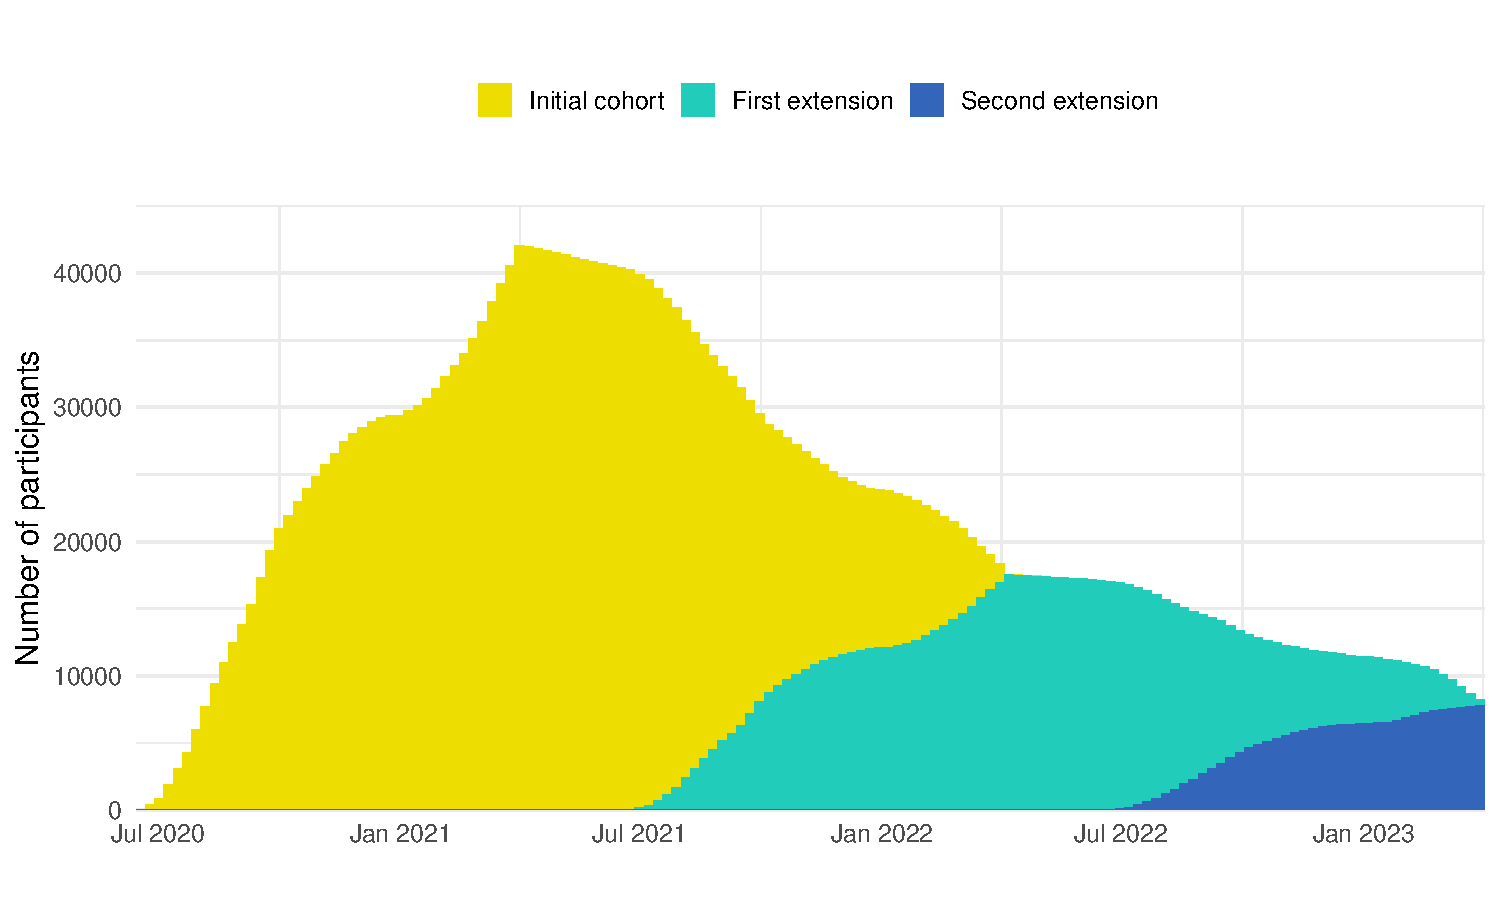
\includegraphics[width=\textwidth]{participants.pdf}
    \caption[Number of participants actively enrolled in SIREN by recruitment status, June 2020 to March 2023]{Number of participants actively enrolled in SIREN by recruitment status, June 2020 to March 2023.}\label{fig:sirenparticipants}
\end{figure}

\subsection{Information collected}

COVID-19 vaccination information, and results from PCR and antibody testing were collected centrally by UKHSA and linked to SIREN participant responses. Results from PCR testing undertaken for other reasons (e.g.\ symptomatic testing, contact tracing, etc.) or prior to study entry were also included in the linked dataset.

Anti-N (to confirm previous infection) and anti-S (to confirm previous infection and/or response to vaccination) antibody tests were used to identify if participants had an infection prior to initial recruitment into the study. Post-recruitment, information from fortnightly PCR testing was used to identify if an infection has occurred, with the date of a positive PCR test used as a proxy for the onset of infection.

Because of intermittent testing and/or infections clearing within the fortnightly window, participants may have received a positive anti-N result without a positive PCR test. In these cases previous analyses have used the date of a positive antibody result as a proxy for infection, but the gaps in testing (i.e.\ `interval-censoring') could be accounted for with an appropriate methodology. Meanwhile, negative anti-N antibody results provide serological evidence of a participant's infection-na\"{\i}ve status~\parencite{UK_Health_Security_Agency2022-ps}.

Information on sequenced variant, cycle threshold (Ct) values, and T-cell counts were available for a subset of SIREN study participants. Sequencing data can be used to determine COVID-19 variant and SIREN sequences were cross-referenced with national data to identify variant circulating periods~\parencite{UK_Government2021-ip}. Ct values indicate the concentration of viral genetic material in a sample, with low Ct values (corresponding to a high viral load) indicating acute disease and high infectivity~\parencite{Public_Health_England2020-it}. However, Ct values are not comparable between different assays and vary considerably according to sampling procedure and laboratory set-up~\parencite{Dahdouh2021-jk}. Alongside antibodies, T-cells provide protection against SARS-CoV-2 infection, and the T-cell immunity induced by vaccination and natural infection was measured and characterised in a sub-study of SIREN participants~\parencite{Angyal2022-nl}.

\subsection{Characteristics of study population at enrolment}

Demographic characteristics of the study population were self-reported at enrolment and included:\ age, gender identity, ethnicity, region of residence, occupational setting, staff type, medical conditions, and household structure. The linked testing and vaccination data included:\ PCR and antibody dates and results, and vaccination dose, date, and manufacturer (with most receiving mRNA vaccines).

As shown in Figure~\ref{fig:occupation_household} panel A, the majority of participants who enrolled in the study reported female gender identity, and most were employed as nurses, doctors, or in other patient-facing roles. Most were aged between aged between 25--65, and among these the majority lived with others (other adults, or both adults and children) (Figure~\ref{fig:occupation_household} panel B).

\begin{figure}[htbp!]
    \centering
    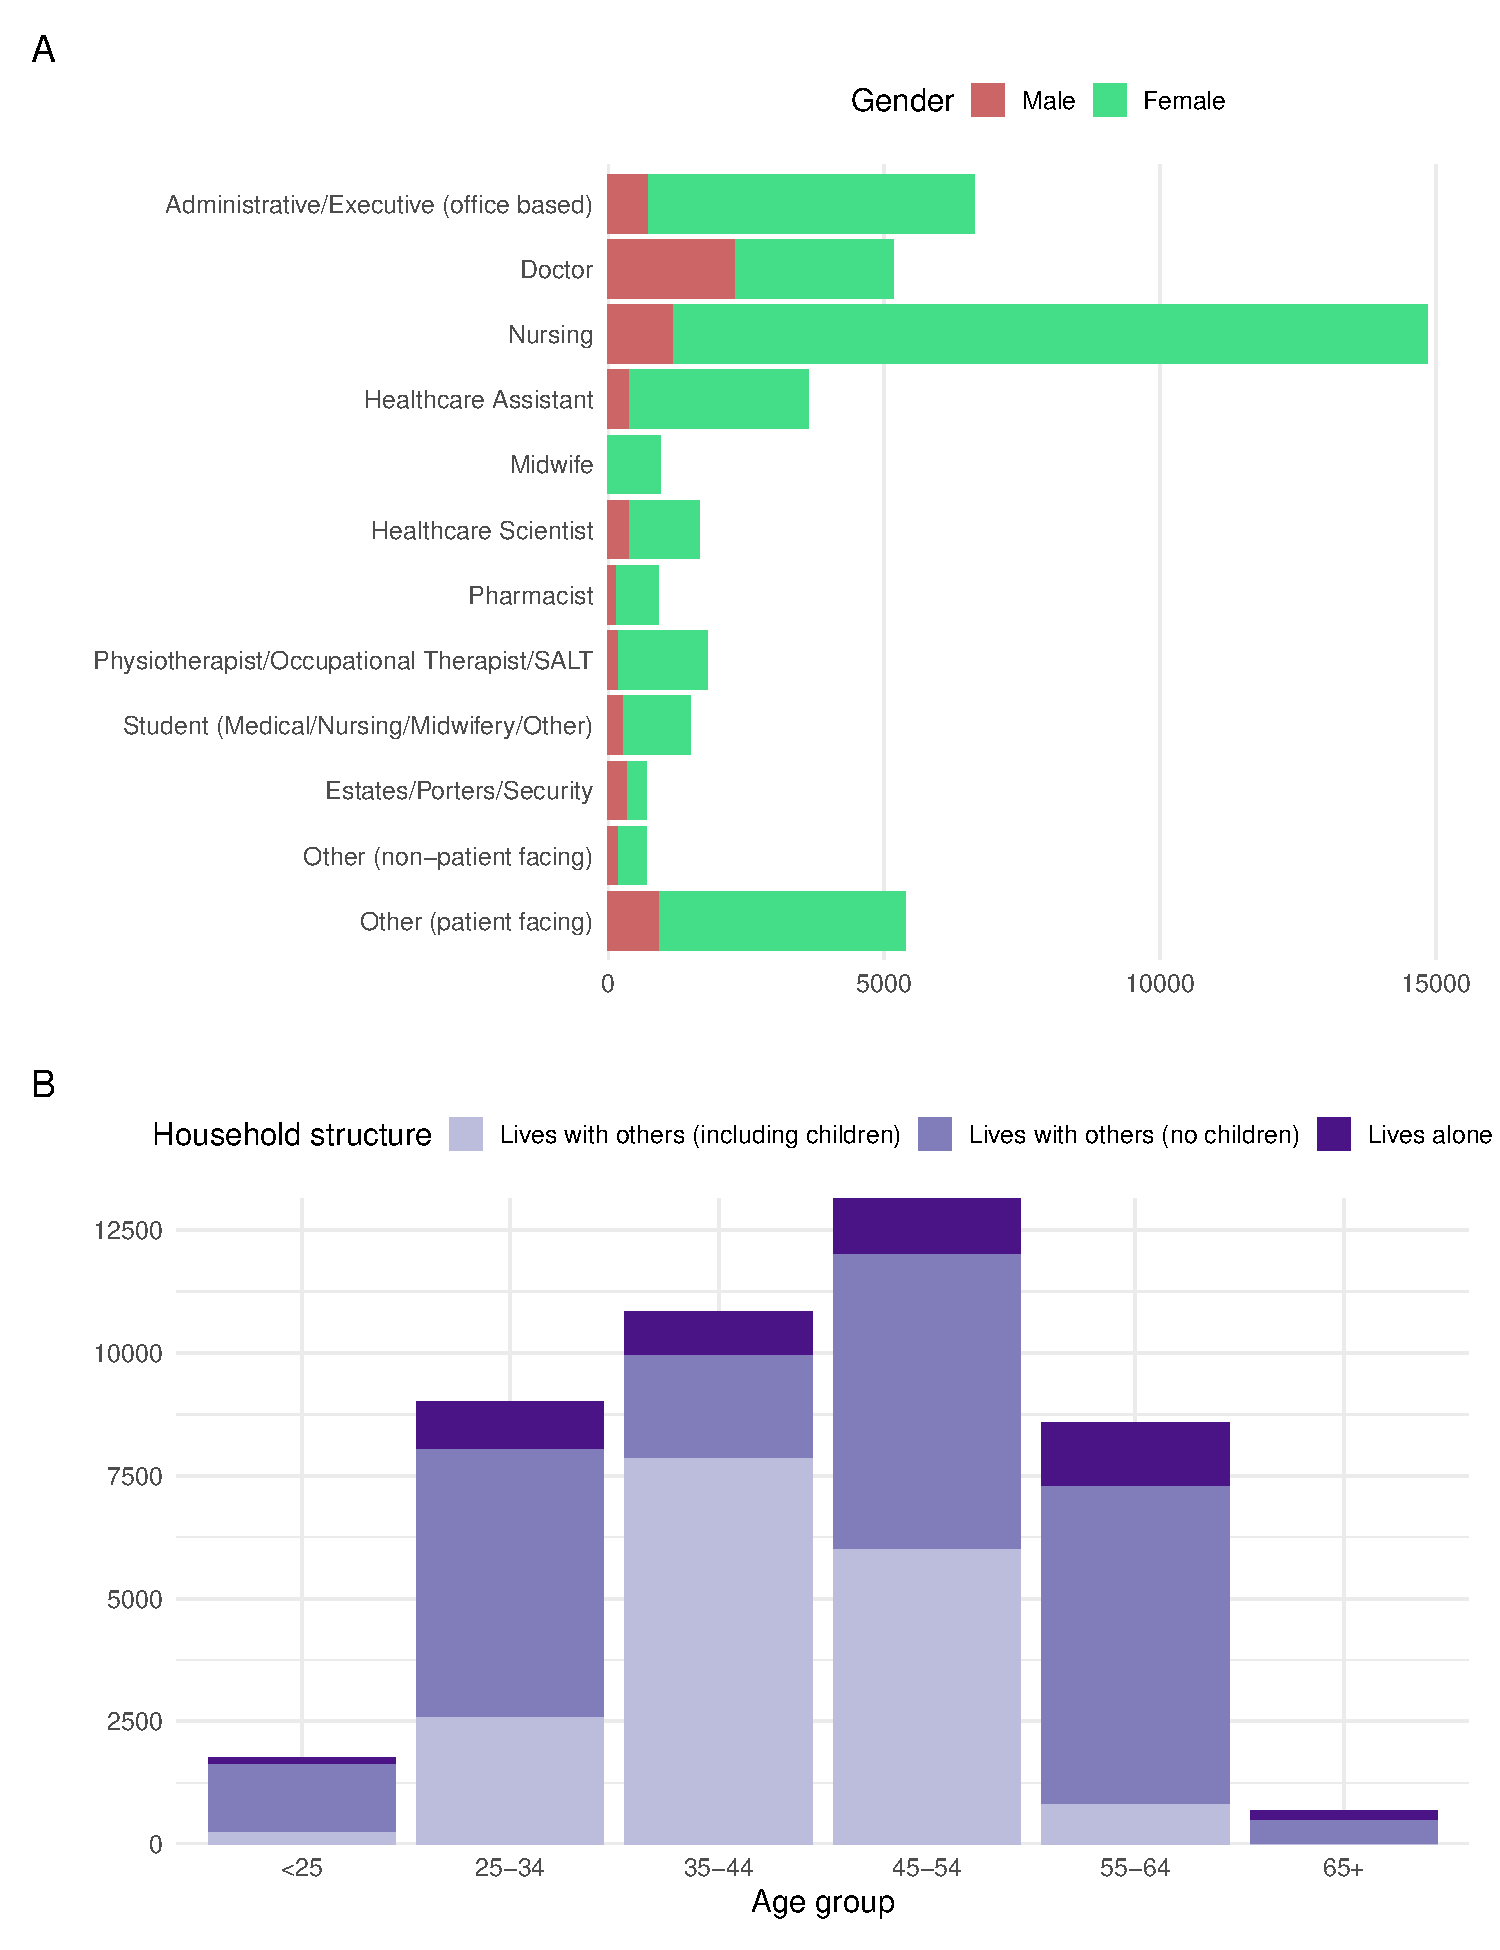
\includegraphics[width=\textwidth]{occupation_household.pdf}
    \caption[SIREN participant demographics, by occupation and gender identity and age group and household structure]{SIREN participant demographics, by occupation and gender identity (panel A) and age group and household structure (panel B).}\label{fig:occupation_household}
\end{figure}

Most study participants were of white ethnicity (87.8\%), and the greatest proportion were from the South of England (South West, South East or London), with smaller numbers of participants in the North East. Three-quarters (75\%) had no chronic medical conditions, although 2.2\% ($n = 969$) reported immunosuppression. Compared to the UK population, participants for whom deprivation information was available lived in less socio-economically deprived areas on average:\ 25.6\% in the least deprived quintile and 11.4\% in the most deprived quintile (Table~\ref{tab:siren_demographics}).

The cohort broadly reflected the demography of UK healthcare workers and whilst the demographic characteristics of the cohort did not differ greatly between the initial cohort and first extension, younger people (aged <25 and 25--34) were particularly under-represented in the second extension (Table~\ref{tab:siren_demographics}).

\subsection{Infections}

Figure~\ref{fig:sireninfections} shows the weekly number of new COVID-19 infections detected through fortnightly PCR testing among SIREN participants over the course of the study. Peaks in the number of new infections appear soon after a change in the predominant circulating variant (inferred from those with sequencing information available) and coincide with peaks in infections detected among the UK population~\parencite{UK_Government2021-ip}.

\begin{figure}[htbp!]
    \centering
    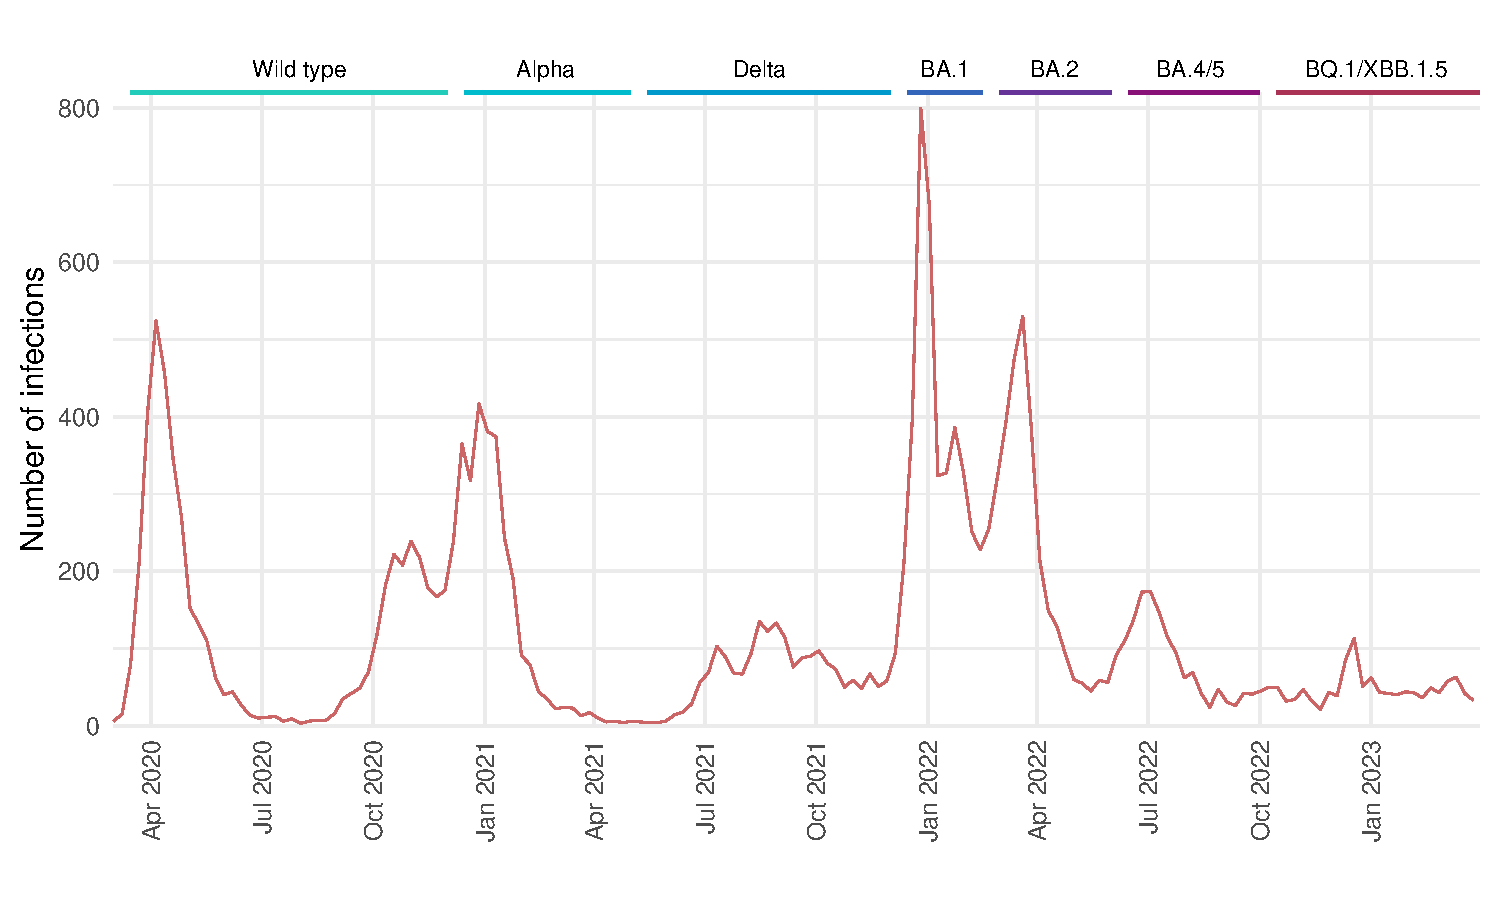
\includegraphics[width=\textwidth]{infections.pdf}
    \caption[Weekly number of new COVID-19 infections detected among SIREN participants, June 2020 to March 2023]{Weekly number of new COVID-19 infections detected among SIREN participants, June 2020 to March 2023. Predominant circulating variant(s) are indicated above.}\label{fig:sireninfections}
\end{figure}

Questionnaires completed by participants within a 14-day window of a positive PCR test (to minimise recall-bias) were used to distinguish between infections with and without COVID-19 symptoms. For this investigation, infections were grouped into two categories based on reported symptoms:\ COVID-19-specific symptoms (any of:\ cough, fever, sore throat, anosmia (loss of smell), and/or dysgeusia (loss of taste)), and asymptomatic for COVID-19 (absence of symptoms, or only non-specific symptoms such as fatigue and muscle ache).

Symptoms varied according to variant, with a greater proportion of participants reporting COVID-19 symptoms during the Delta, BA.1, and BA.2 variant circulating periods compared to the Wild type or later variants (Figure~\ref{fig:symptoms_age_sex} panel A). Prevalence of symptomatic infection did not differ by gender, but younger participants were more likely to report COVID-19-specific symptoms as compared to older participants (Figure~\ref{fig:symptoms_age_sex} panel B).
\newline
\newline

\begin{figure}[htbp!]
    \centering
    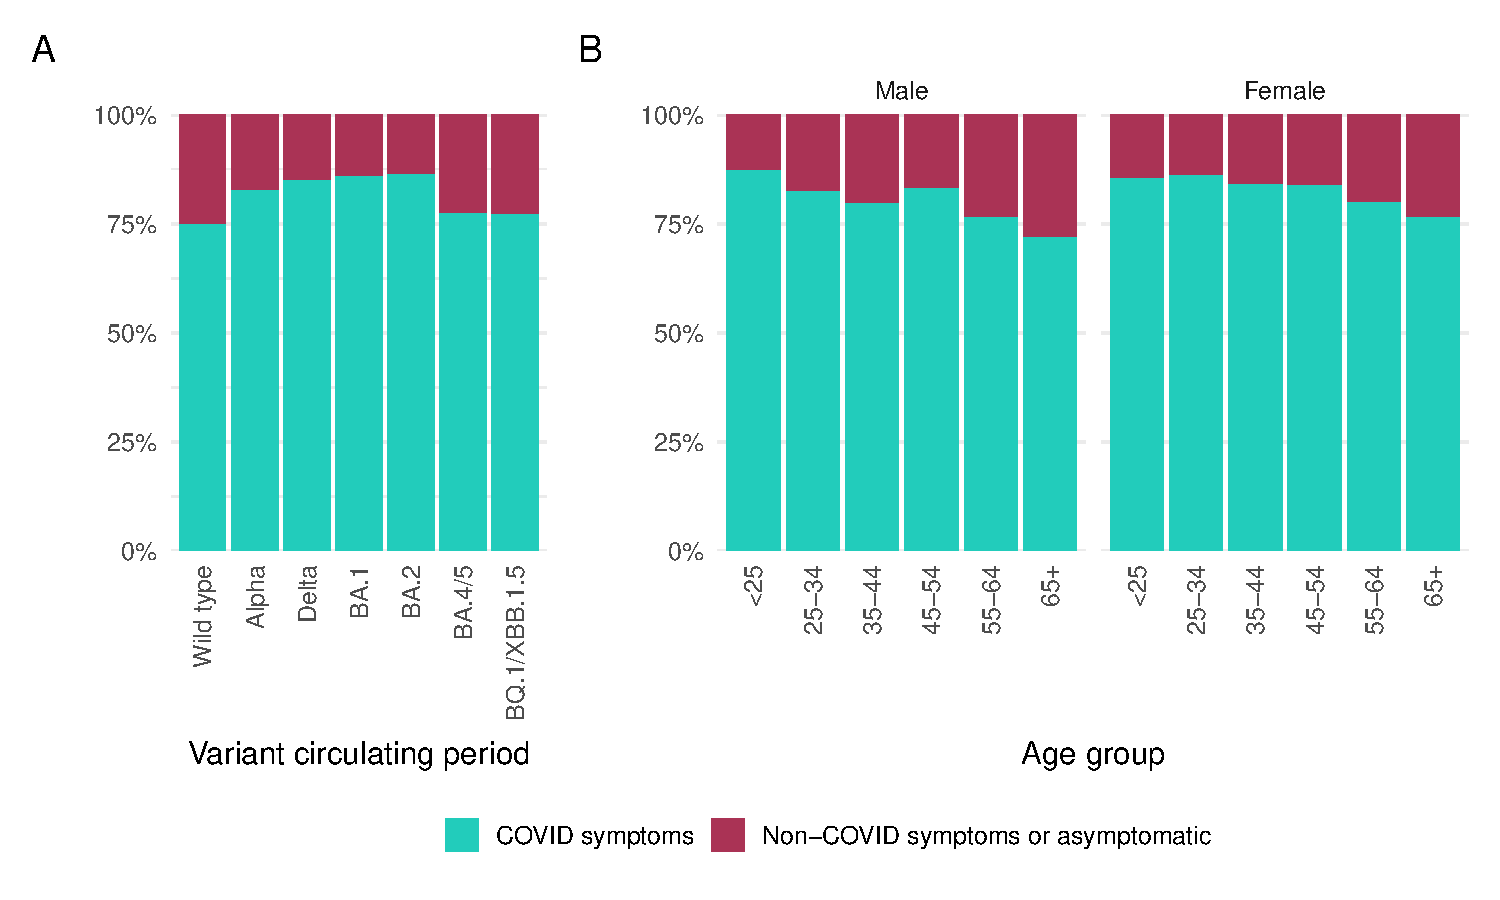
\includegraphics[width=\textwidth]{symptoms_age_sex.pdf}
    \caption[Self-reported symptoms among SIREN participants testing positive for COVID-19 between June 2020 to March 2023, by circulating variant period, and age and gender]{Self-reported symptoms among SIREN participants testing positive for COVID-19 between June 2020 to March 2023, by circulating variant period (panel A), and age and gender (panel B).}\label{fig:symptoms_age_sex}
\end{figure}

\subsection{Vaccination}

Primary (first and second dose), and first booster (third dose) COVID-19 vaccine coverage was high and rapid, with the majority of participants accepting a vaccine within 2-months of vaccine availability (Figure~\ref{fig:prop_vaccinated}, panels A and B). Coverage of the second booster (fourth dose) was notably slower and less widespread, with a smaller proportion of participants receiving a fourth dose within 60 days of vaccine availability (64.3\%), compared to third doses (83.0\%). Fourth dose vaccine coverage within 60 days was particularly low in Scotland compared to other UK regions (Figure~\ref{fig:vaccination_history_region}).

\begin{figure}[htbp!]
    \centering
    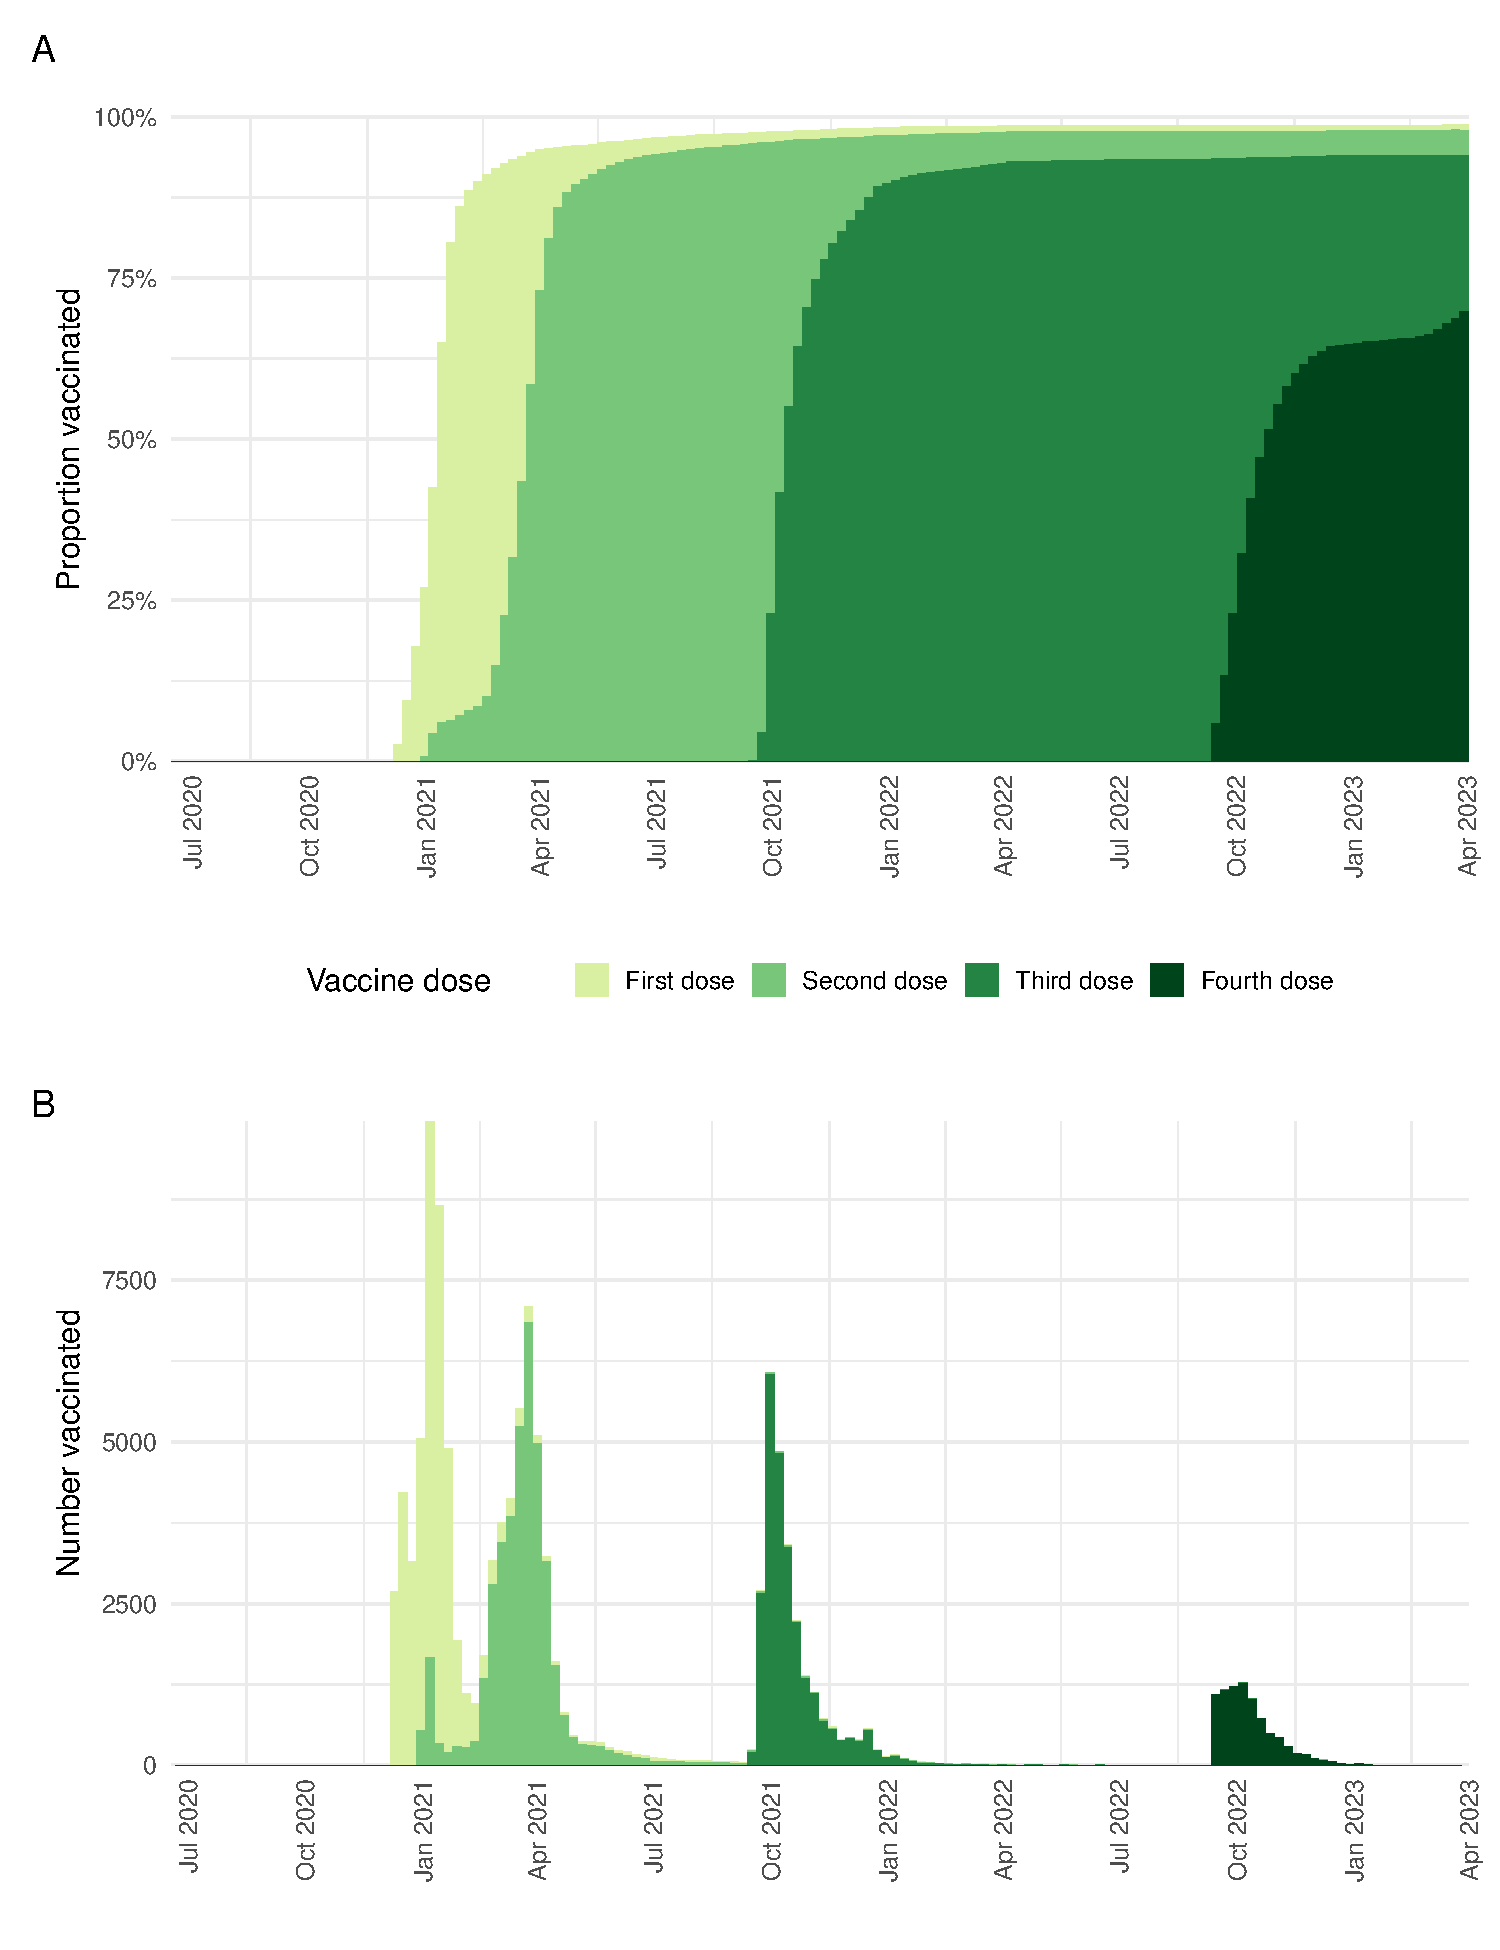
\includegraphics[width=\textwidth]{proportion_vaccinated.pdf}
    \caption[Proportion of SIREN participants vaccinated and number of participants vaccinated each week, by vaccine dose, June 2020 to March 2023]{Proportion of SIREN participants vaccinated (panel A) and number of participants vaccinated each week (panel B), by vaccine dose, June 2020 to March 2023.}\label{fig:prop_vaccinated}
\end{figure}

\begin{figure}[htbp!]
    \centering
    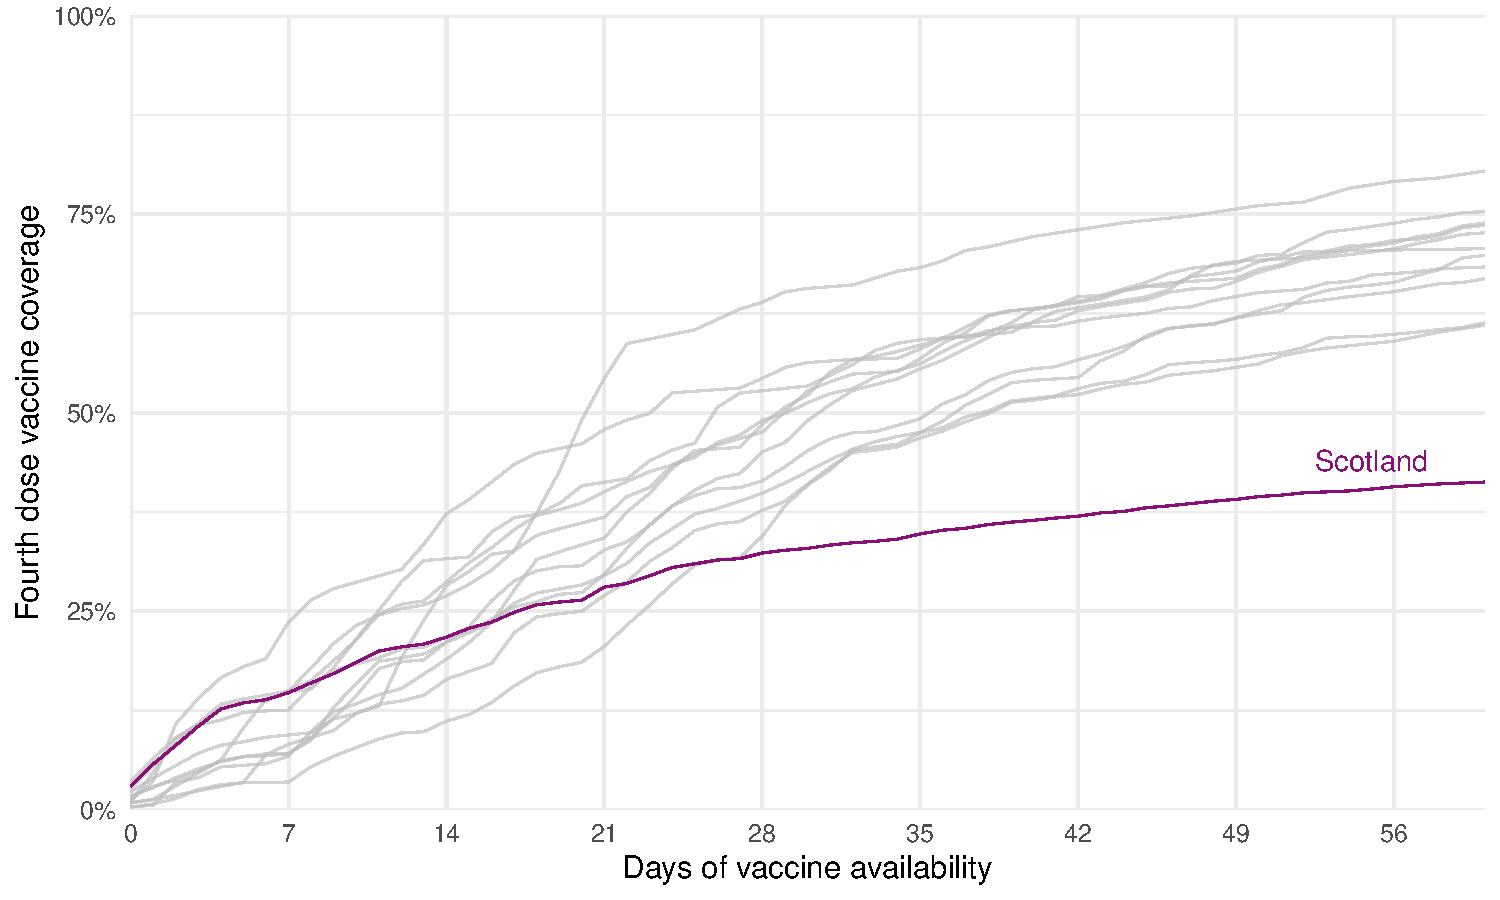
\includegraphics[width=\textwidth]{vaccination_history_region.pdf}
    \caption[Fourth dose vaccine coverage among SIREN participants within 60 days of vaccine availability, by region of residence]{Fourth dose vaccine coverage among SIREN participants within 60 days of vaccine availability, by region of residence.}\label{fig:vaccination_history_region}
\end{figure}

Younger participants were less likely to receive a fourth dose (\var{prop_vu_2534}\% for those aged 25--34 compared to \var{prop_vu_65}\% for those aged over 65) (Figure~\ref{fig:vaccination_demog}, Panel A), whereas infection-na\"{\i}ve participants were slightly more likely to receive a fourth dose than those with a recent COVID-19 infection (\var{prop_inf_naive}\% vs.\ \var{prop_inf_06}\%) (Figure~\ref{fig:vaccination_demog}, Panel B). Fourth dose vaccine coverage by other demographic characteristics is shown in Table~\ref{tab:siren_vaccine_uptake}.

\begin{figure}[htbp!]
    \centering
    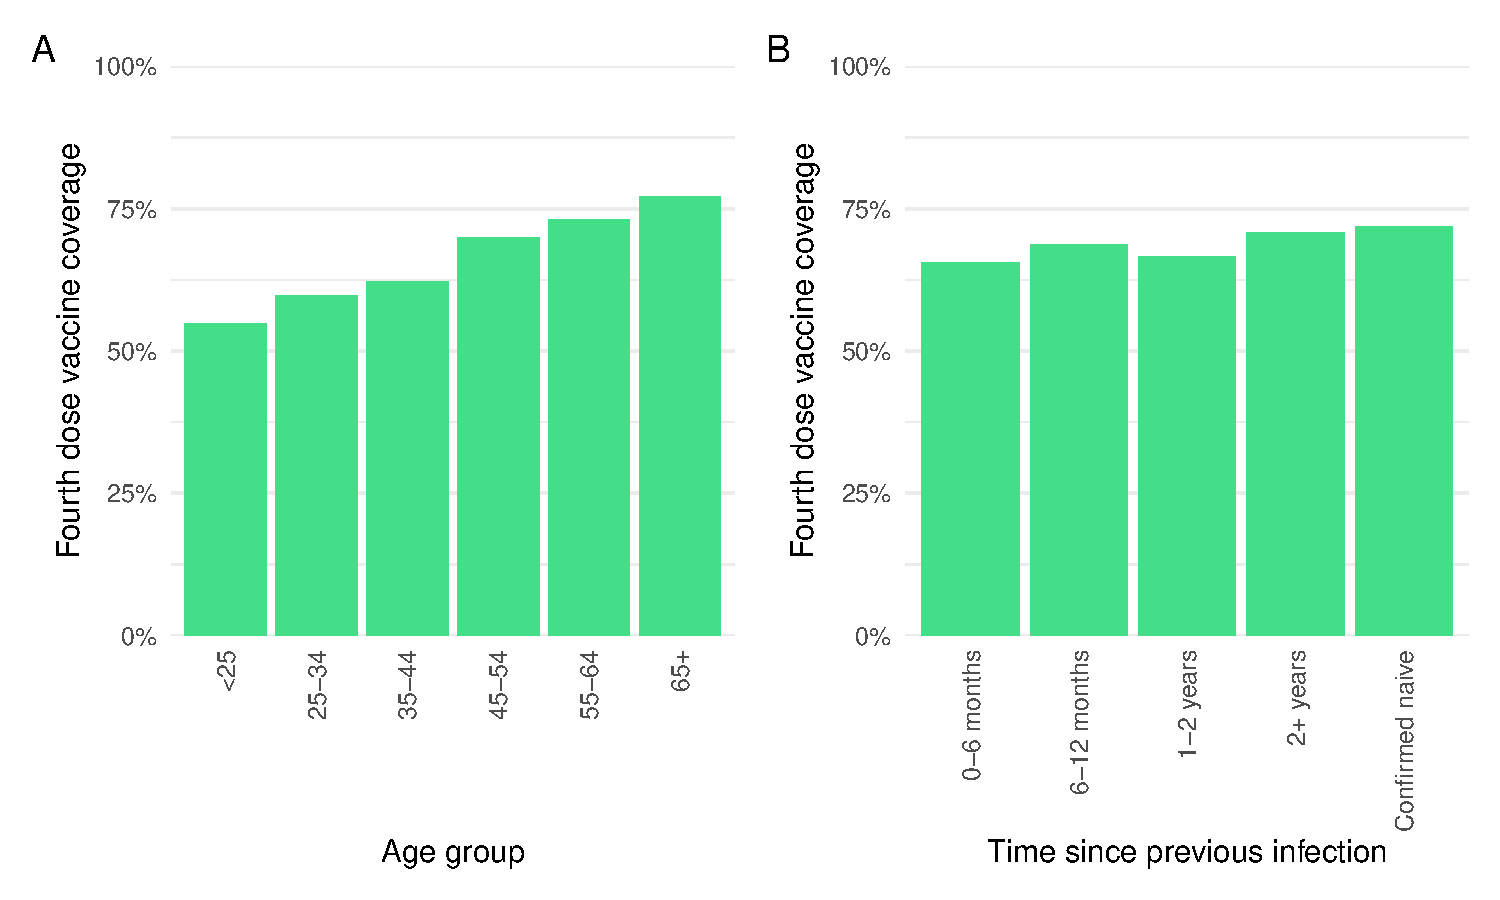
\includegraphics[width=\textwidth]{vaccination_demog.pdf}
    \caption[Fourth dose vaccine coverage among SIREN participants by age group and time since previous infection]{Fourth dose vaccine coverage among SIREN participants by age group (panel A) and time since previous infection (panel B).}\label{fig:vaccination_demog}
\end{figure}

\subsection{Fortnightly testing}\label{sec:fortnightly-testing}

PCR testing in SIREN was performed through several means, which varied by site. Testing pathways included:\ on-site nurse-led testing, self-testing with samples being dropped off by participants at an on-site drop-box, and self-testing with participants returning the samples by post ($n=3,500$ individuals).

Figure~\ref{fig:siren_timeline} shows a timeline of participation in the SIREN study and vaccination status at each time point for a subset of randomly selected participants. The date of enrolment and PCR test dates are overlaid onto the timeline, demonstrating substantial variation among participants; some tested frequently and regularly, whilst others tested at irregular intervals and/or missed several tests.

\begin{figure}[htbp!]
    \centering
    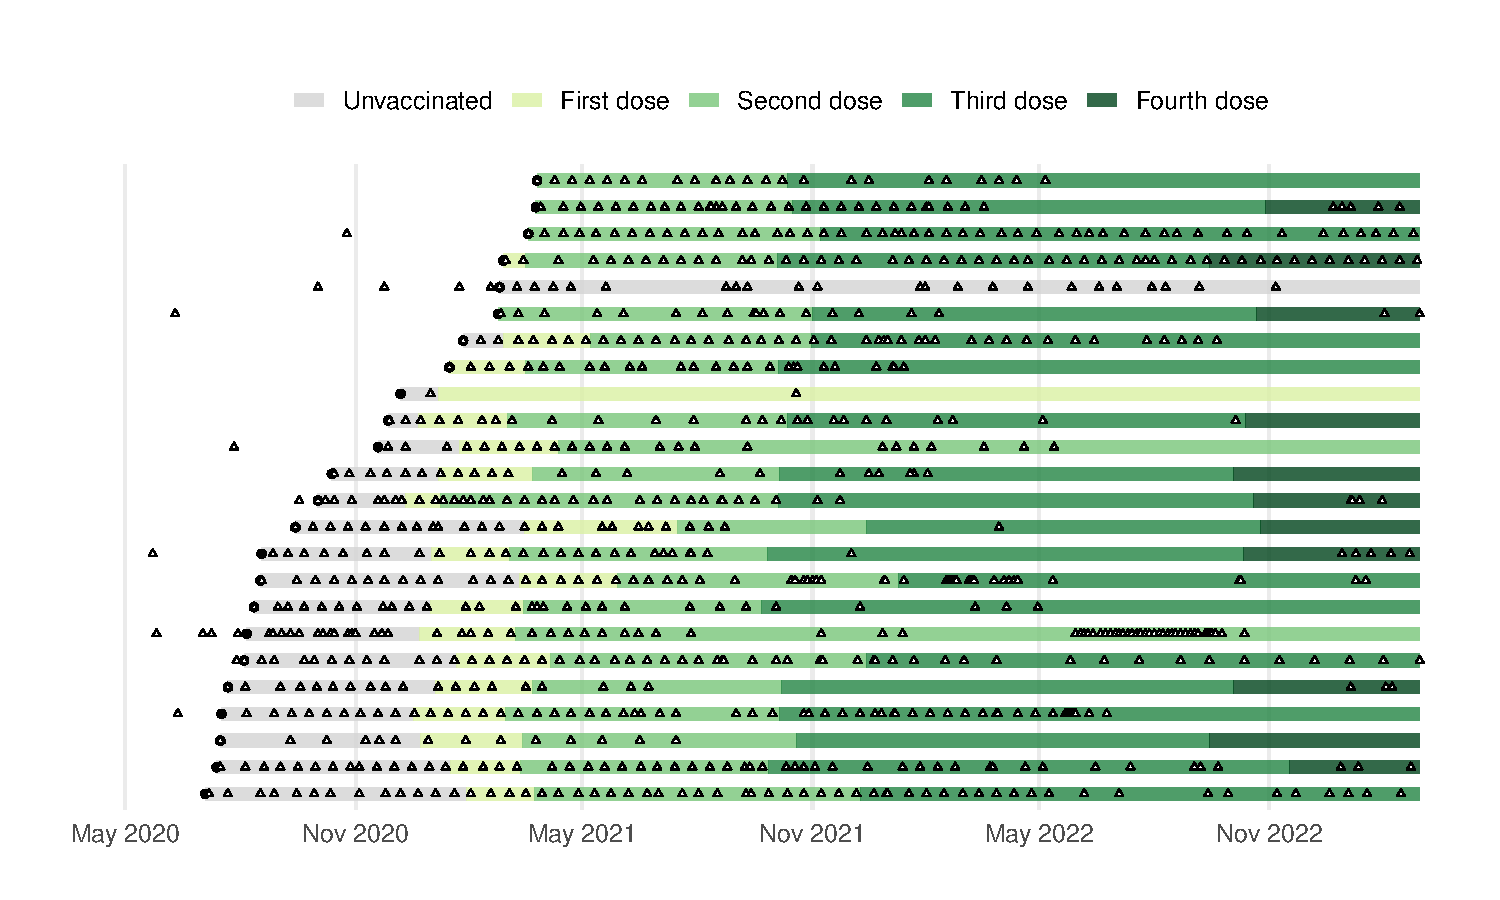
\includegraphics[width=\textwidth]{siren_timeline.pdf}
    \caption[Timeline of study participation and vaccination status for randomly selected SIREN participants, June 2020 to March 2023]{Timeline of study participation and vaccination status for randomly selected SIREN participants, June 2020 to March 2023. Key:\ enrolment ($\bullet$), PCR testing ($\triangle$).}\label{fig:siren_timeline}
\end{figure}

Whilst participants may have missed tests for a variety of reasons, including annual leave, shift changes, or illness, there was some evidence of testing fatigue over time:\ \var{prop_ft_wt}\% of participants underwent PCR testing according to the fortnightly schedule during the Wild type variant circulating period, and \var{prop_ft_delta}\% during the Delta period, but this reduced to \var{prop_ft_bq}\% during the BQ.1/XBB.1.5 period (Figure~\ref{fig:fortnightly_schedule}).

Lower adherence to the fortnightly testing schedule coincided with the removal of non-pharmaceutical interventions, and return to more normal population mixing~\parencite{Department_of_Health_and_Social_Care2020-ez, Smith2022-iv}.
\newline

\begin{figure}[htbp!]
    \centering
    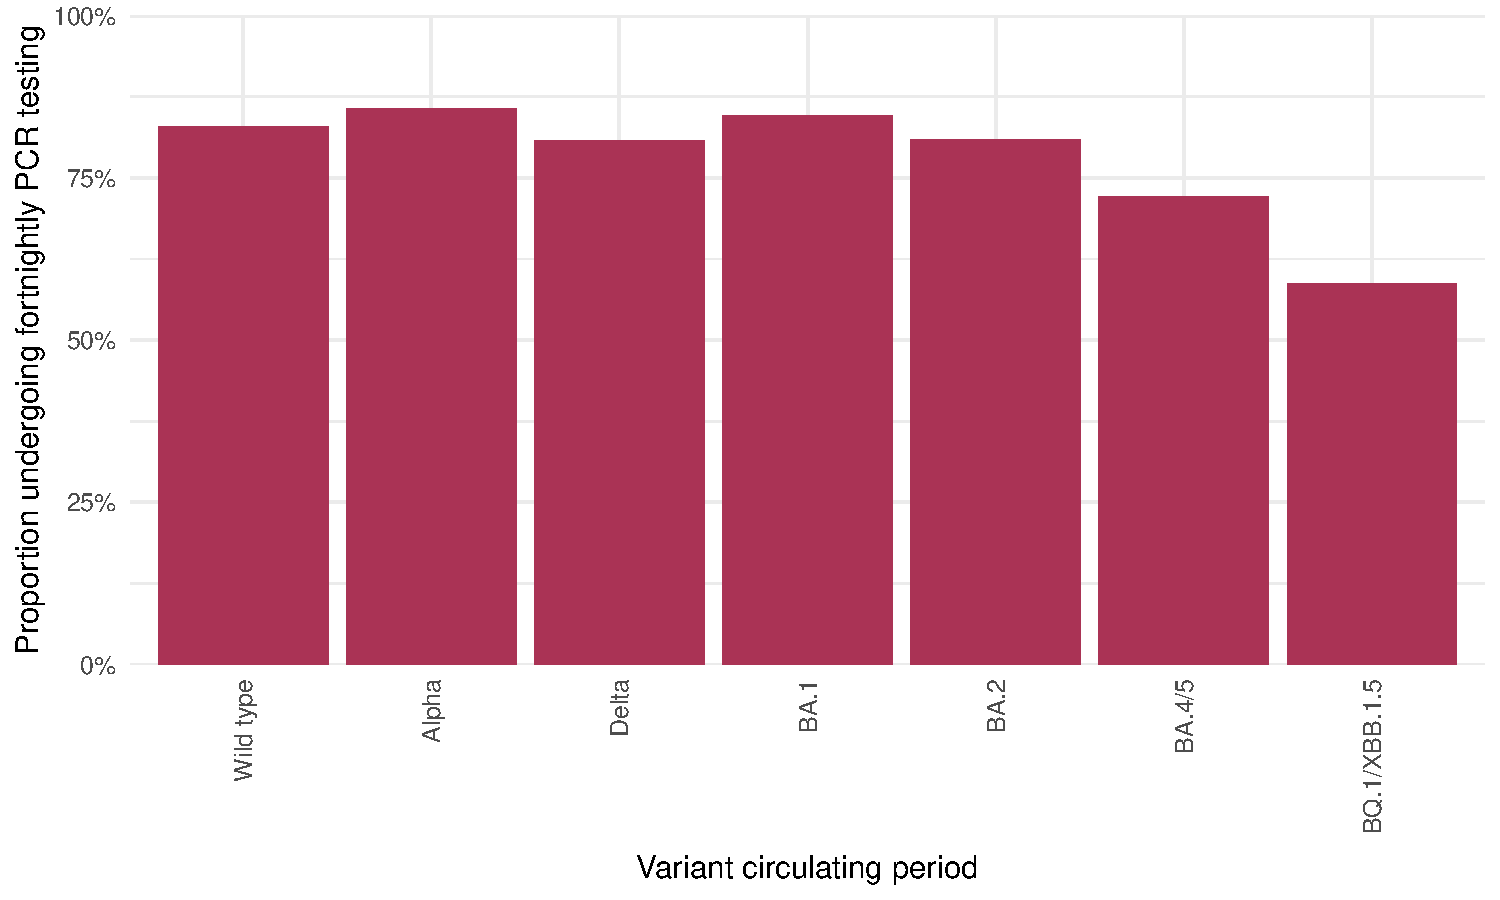
\includegraphics[width=\textwidth]{fortnightly_schedule.pdf}
    \caption[Proportion of enrolled SIREN participants undergoing PCR testing on a fortnightly schedule, by variant circulating period]{Proportion of enrolled SIREN participants undergoing PCR testing on a fortnightly schedule, by variant circulating period.}\label{fig:fortnightly_schedule}
\end{figure}

\subsection{Cox proportional hazards models}

Stratified Cox proportional hazards models, described in Section~\ref{sec:cox-model}, were applied to the SIREN study data in two `interim analyses':\ firstly to estimate protection from prior infection and vaccination during the Alpha and Delta variant circulating period; and secondly to estimate protection of first booster doses and previous infection against Omicron sub-variants compared to Delta.

The main findings of these analyses are included in Appendix~\ref{appendix:siren-cox-models}, and further details can be found in the two publications~\parencite{Hall2022-ep, Hall2024-ai}. These analyses supported the use of booster vaccination to sustain immunity, and highlighted the challenges posed by new variants.

\section{Cohort study design}\label{sec:cohort-study-design}

\subsection{Biases in vaccine effectiveness studies}

\textbf{Test-negative case-control} study designs are routinely used to assess vaccine effectiveness, both for influenza and COVID-19~\parencite{Andrews2022-qd, Dean2021-qw, Lopez_Bernal2021-gt}. Latent healthcare-seeking behaviour may influence vaccine uptake, infection, and testing, as shown in Figure~\ref{fig:test-neg} panel A. By conditioning on testing, the test-negative case-control study design controls for this potential source of bias, as shown in Figure~\ref{fig:test-neg} panel B.

Despite controlling for healthcare-seeking behaviour, a test-negative case-control study may be subject to several other uncontrolled biases~\parencite{Shi2023-ic, Sullivan2016-io}. In particular, `collider stratification bias' can arise if, say, workplace testing policies require unvaccinated individuals to test on a more regular basis (shown by the blue arrow in Figure~\ref{fig:test-neg} panel B); or alternatively, if vaccinated individuals are less likely to be symptomatic, and hence less likely to get tested for infection (shown by the red arrow in Figure~\ref{fig:test-neg} panel B).

\textbf{Cohort} study designs, where people test according to a pre-determined observation scheme, improve on the test-negative case-control study design by addressing the specific `collider stratification' biases whilst still controlling for health-seeking behaviour. The corresponding causal diagram for a cohort study design is shown in Figure~\ref{fig:test-neg} panel C. The cohort study design in SIREN also benefits from being able to capture both symptomatic and asymptomatic infection.

Despite accounting for the specific biases described, both study designs remain subject to biases from unmeasured confounding, misclassification, and may suffer from a lack of generalisability.

\begin{figure}[htbp!]
    \centering
    \begin{tikzpicture}
        % x node set with absolute coordinates
        \node (v) at (0,0) {$V$};
        \node (i) [right = of v] {$I$};
        \node (s) [right = of i] {$S$};
        \node (t) [right = of s] {$T$};
        \node (is) [below = of s] {$I^*$};
        \node (h) [above = of s] {$H$};
        \node (l) [above left = 0mm and 30mm of h] {\textsf{A}};

        % Directed edge
        \path (v) edge (i);
        \path (i) edge (s);
        \path (s) edge (t);
        \path (i) edge (is);
        \path (t) edge (is);
        \path (h) edge (v);
        \path (h) edge (i);
        \path (h) edge (t);
    \end{tikzpicture}
    \hspace{1em}
    \begin{tikzpicture}
        % x node set with absolute coordinates
        \node (v) at (0,0) {$V$};
        \node (i) [right = of v] {$I$};
        \node (s) [right = of i] {$S$};
        \node[state] (t) [right = of s] {$T=1$};
        \node (is) [below = of s] {$I^*$};
        \node[state] (h) [above = of s] {$H=1$};
        \node (l) [above left = 0mm and 30mm of h] {\textsf{B}};

        % Directed edge
        \path (v) edge (i);
        \path (i) edge (s);
        \path (s) edge (t);
        \path (i) edge (is);
        \path (t) edge (is);
        \path (v) edge[color = blue, bend left = 35] (t);
        \path (v) edge[color = red, bend left = 30] (s);
    \end{tikzpicture}\vspace{1.5em}
    \begin{tikzpicture}
        % x node set with absolute coordinates
        \node (v) at (0,0) {$V$};
        \node (i) [right = of v] {$I$};
        \node (is) [right = of i] {$I^*$};
        \node[state] (t) [above = of is] {$T = 1$};
        \node (l) [above left = 0mm and 30mm of h] {\textsf{C}};

        % Directed edge
        \path (v) edge (i);
        \path (i) edge (is);
        \path (t) edge (is);
    \end{tikzpicture}\vspace{1em}
    \caption[Causal DAG describing the relationship between vaccination, infection, symptoms, testing, and latent health-seeking behaviour in a test-negative case-control study and a cohort study]{Causal DAG describing the relationship between vaccination ($V$), infection ($I$), observed infection ($I^*$), symptoms ($S$), testing ($T$), and latent health-seeking behaviour ($H$) (panel A), the potential biases which may remain after adjusting for test-seeking behaviour in a test-negative case-control study (panel B), and in a cohort study (panel C).}\label{fig:test-neg}
\end{figure}

\subsection{Intermittent observation}

An additional challenge, specific to observational cohort data, is \textit{intermittent observation} of the underlying process, also termed interval-censoring.

In the Cox proportional hazards models described in Section~\ref{appendix:siren-cox-models} only the positive test information in SIREN was used, with the assumption that participants remained uninfected in the absence of a positive test. However, as described in Section~\ref{sec:censoring-intermittent}, intermittent (and irregular) observation of participants' PCR status could result in infections being undetected.

Adherence to the fortnightly testing schedule during the Wild type, Alpha, Delta, and Omicron BA.1/2 variant circulating periods was high (Figure~\ref{fig:fortnightly_schedule}), so the regular PCR and antibody testing in SIREN was judged to be sufficient to detect the majority of COVID-19 infections. During the BA.4/5 and BQ.1/XBB.1.5 variant circulating periods, however, a greater proportion of participants missed PCR tests and there was less frequent monitoring of antibodies, which may limit the validity of Cox proportional hazards model estimates during this period. To address the challenge of intermittent observation multi-state models can be considered. Multi-state models will correctly account for interval-censoring when this censoring is non-informative~\parencite{van-den-Hout2016-xy}.

At the start of autumn 2022, in anticipation of a new wave of SARS-CoV-2 infections, second vaccine boosters (i.e.\ fourth doses) were offered to healthcare workers alongside their seasonal influenza vaccinations. In the next section I develop multi-state models which are applied to estimate fourth dose vaccine effectiveness against SARS-CoV-2 infection during the autumn/winter 2022/23 period.

\section{Multi-state models}\label{sec:siren-msm}

In Section~\ref{sec:multi-state-models} I described how parameters related to infection may be estimated by fitting a multi-state model to the set of observed state transitions for a group of individuals. In this section I describe several `SIR-type' multi-state models which account for the specific challenges of intermittent observation and misclassification in observational cohort data.

I apply these models to the SIREN data to estimate the protection of second booster vaccination and prior SARS-CoV-2 infection against infection (both symptomatic and asymptomatic), and mean duration of PCR positivity among triple-vaccinated healthcare workers between September 2022 and March 2023 (i.e.\ the period of Omicron BA.4/5 and BQ.1/XBB.1.5 sub-variant circulation).

The public health research question was whether healthcare workers should be routinely offered autumn vaccine boosters, given the short-term nature of protection and uncertainty about future variant emergence.

\subsection{Multi-state model frameworks}

SIREN participants test according to pre-specified dates, with observations representing testing rather than the occurrence of infection. For an individual with a PCR-negative status at time $L$ and PCR-positive status at time $R$, infection is assumed to occur at some time $T \in [0,\infty)$ during the time interval $(L,R]$. The infection time is therefore interval-censored, $T \in (L,R]$. If the time intervals are fixed in advance then this interval censoring is independent of $T$, formally~\parencite{van-den-Hout2016-xy}:
%
\[
    \Pr(L < T \leq R \mid L=l, R=r) = \Pr(l < T \leq r)
\]

As independent interval-censoring implies a non-informative observation scheme, multi-state models are a suitable choice for this analysis~\parencite{van-den-Hout2016-xy}. These models implicitly account for incomplete testing (i.e.\ gaps in an individual's testing history), without the assumption that an individual remains uninfected despite not testing. Since observation in SIREN occurs at fixed 2-weekly time intervals, continuous-time multi-state models were used which allow for changes of state (from susceptible to infected, and infected to recovered) to occur at any point during the time interval.

\subsubsection{Two-state model}

A two-state `SI' model, where individuals move between a susceptible (S) and an infected (I) state, is one of the simplest forms of multi-state model. Individuals with a negative test result (indicating lack of infection) are observed to be currently in the susceptible state, and those with a positive test result (indicating infection) are observed to be currently in the infected state. As shown in Figure~\ref{fig:two-state-model}, the model is defined by transition intensities $q_{12}$ and $q_{21}$ between these two states, and covariate effects may be included on these transitions.

\begin{figure}[htbp!]
    \centering
    \begin{tikzpicture}
        % x node set with absolute coordinates
        \node[cstate] (s) at (0,0) {$S$};

        % y node set relative to x
        \node[cstate] (i) [right =of s] {$I$};

        % Directed edge
        \path (s) edge[bend left=30] node[above] {$q_{12}$} (i);
        \path (i) edge[bend left=30] node[below] {$q_{21}$} (s);

        % Title
        \node[font=\bfseries, left=20mm of s] at ($(s)!0.5!(i)$) (titles)  {Negative test};
        \node[below=0mm of titles] (sus)  {(Susceptible)};
        \node[font=\bfseries, right=20mm of i] at ($(s)!0.5!(i)$) (titlei)  {Positive test};
        \node[below=0mm of titlei] (inf)  {(Infected)};

    \end{tikzpicture}
    \caption[Two-state `SI' model]{Two-state `SI' model, defined by transition intensities $q_{12}$ and $q_{21}$.}\label{fig:two-state-model}
\end{figure}

\subsubsection{Three-state model}

Immediately following recovery from infection there is typically very little risk of reinfection~\parencite{Hall2021-rh}. Whilst this `convalescence' period can be represented through a covariate in the two-state model, an extension to a three-state `SIR' model is also possible through the inclusion of a recovery state (R). Within the recovery state participants are not at risk of infection and must first progress to the susceptible state, as shown in Figure~\ref{fig:three-state-model}.

\begin{figure}[htbp!]
    \centering
    \begin{tikzpicture}
        % x node set with absolute coordinates
        \node[cstate] (s) at (0,0) {$S$};

        % y node set relative to x
        \node[cstate] (i) [right =of s] {$I$};
        \node[cstate] (r) [right =of i] {$R$};

        % Directed edge
        \path (s) edge node[above] {$q_{12}$} (i);
        \path (i) edge node[above] {$q_{23}$} (r);
        \path (r) edge[bend left=40] node[below] {$q_{31}$} (s);

    \end{tikzpicture}
    \caption[Three-state `SIR' model]{Three-state `SIR' model defined by transition intensities $q_{12}$, $q_{23}$, and $q_{31}$.}\label{fig:three-state-model}
\end{figure}

\subsubsection{Symptom status model}

Self-reported symptoms information may be used to classify infections as symptomatic/asymptomatic and these states modelled as separate outcomes, $I_s$ and $I_a$, as shown in Figure~\ref{fig:symptom-model}. Whilst $q_{12}$ and $q_{13}$ represent the incidence of asymptomatic and symptomatic infection, typically of greater interest in these models are the covariate effects on these transition intensities, and the mean sojourn time in each state.

\begin{figure}[htbp!]
    \centering
    \begin{tikzpicture}
        % x node set with absolute coordinates
        \node[cstate] (s) (0,0) {$S$};

        % y node set relative to x
        \node[cstate] (ia) [right =15mm of s,yshift=1cm] {$I_a$};
        \node[cstate] (is) [right =15mm of s,yshift=-1cm] {$I_s$};

        % Directed edge
        \path (s) edge node[below, pos = 0.6] {$q_{12}$} (ia);
        \path (s) edge node[above, pos = 0.6] {$q_{13}$} (is);
        \path (ia) edge[bend left=-40] node[above] {$q_{21}$} (s);
        \path (is) edge[bend left=40] node[below] {$q_{31}$} (s);

        % Title
        \node[font=\bfseries, left=20mm of s] at ($(s)!0.5!(ia)$) (titles)  {Negative PCR test};
        \node[below=0mm of titles] (sus)  {(Susceptible)};
        \node[font=\bfseries, right=25mm of s] (titlei)  {Positive PCR test};
        \node[above=4mm of titlei] (infa)  {(Asymptomatic)};
        \node[below=4mm of titlei] (infs)  {(Symptomatic)};

    \end{tikzpicture}
    \caption[Symptom status multi-state model]{Symptom status multi-state model defined by transition intensities $q_{12}$, $q_{13}$, $q_{21}$, and $q_{31}$.}\label{fig:symptom-model}
\end{figure}

\subsubsection{Semi-Markov model}

The models considered so far in this section are Markov, where transition to the next state does not depend on the time spent in a state. Relaxing this assumption may allow the model to better represent recovery from a disease, as transition from the $I$ to the $S$ state typically becomes more likely as time progresses i.e.\ for the two-state model, allowing $q_{21}$ to depend on the time spent in state $I$.

In a semi-Markov multi-state model, transition intensities depend on the time spent in the current state, but not on previous states:
%
\[
    q_{rs}(t; \mathcal{X}_t) = q_{rs}(t - t_r)
\]

where $\mathcal{X}_t$ is the observation history of the process up to time $t$, and $t_r$ is the time of entry into the current state $r$~\parencite{Jackson2011-ry}.

To achieve this in the two-state model the $I$ state is sub-divided into two `hidden' states, with paths through these states representing short-stayers ($S \rightarrow I_1 \rightarrow S$) and long-stayers ($S \rightarrow I_1 \rightarrow I_2 \rightarrow S$), as shown in Figure~\ref{fig:semi-markov-model}.

\begin{figure}[htbp!]
    \centering
    \begin{tikzpicture}
        % x node set with absolute coordinates
        \node[cstate] (s) at (0,0) {$S$};

        % y node set relative to x
        \node[cstate] (i1) [right =15mm of s] {$I_1$};
        \node[cstate] (i2) [right =of i1] {$I_2$};

        % Directed edge
        \path (s) edge node[above] {$q_{12}$} (i1);
        \path (i1) edge node[above] {$\lambda_1$} (i2);
        \path (i1) edge[bend left=60] node[above] {$\mu_1$} (s);
        \path (i2) edge[bend left=60] node[below] {$\mu_2$} (s);

        % Box
        \node[draw=blue,dashed,fit=(i1) (i2), inner sep=0.2cm, label={[text=blue]30:{$I$}}] (i) {};

    \end{tikzpicture}
    \caption[Semi-Markov multi-state model with two hidden states]{Semi-Markov multi-state model with two hidden states $I_1$ and $I_2$ and associated transition intensities.}\label{fig:semi-markov-model}
\end{figure}

This is equivalent to making the sojourn distribution in the $I$ state more flexible than an exponential distribution, such that the hazard of leaving $I$ depends on how long has been spent there. In this model an individual is a long-stayer with probability ${\lambda_1}/{(\lambda_1 + \mu_1)}$.

% and the sojourn times for short and long-stayers are calculated respectively as:

% \[
%     E(T_{I_1}) = \frac{1}{\mu_1+\lambda_1},\quad\quad
%     E(T_{I_1}) + E(T_{I_2}) =\frac{1}{\mu_1+\lambda_1} + \frac{1}{\mu_2}
% \]

\subsubsection{Misclassification model}

Multi-state models may also be extended to account for misclassification in the observed states, reflecting the non-zero probability of an infected person being observed as uninfected, and vice-versa. The Coronavirus Infection Survey (CIS)\nomenclature[z]{CIS}{Coronavirus Infection Survey} previously estimated the test sensitivity (true-positive rate) of SARS-CoV-2 PCR tests to be 99.9\%, and test specificity (true-negative rate) to be between 85--98\%~\parencite{Wei2023-ry}.

These probabilities may be included through a hidden-Markov, or misclassification model, with true positive ($P$), true negative ($N$), observed PCR-negative ($S$), and observed PCR-positive ($I$) states. The corresponding misclassification rates $\Pr(I \mid N)$ and $\Pr(S \mid P)$ may be fixed (as shown in Figure~\ref{fig:hidden-markov-model}) or may exist as unknown parameters to be estimated.

\begin{figure}[htbp!]
    \centering
    \begin{tikzpicture}
        % x node set with absolute coordinates
        \node[cstate] (s) at (0,0) {$N$};
        \node[cstate] (i) [right =25mm of s] {$P$};
        \node[cstate] (oi) [above = 15mm of i] {$I$};
        \node[cstate] (os) [above = 15mm of s] {$S$};

        % Directed edge
        \path (s) edge node[above] {$q_{12}$} (i);
        \path (i) edge[bend left=40] node[below] {$q_{21}$} (s);

        \path (s) edge node[anchor=center, fill=white] {$0.999$} (os);
        \path (i) edge node[anchor=center, fill=white] {$0.91$} (oi);
        \path (s) edge[dashed] node[anchor=center, sloped, fill=white, pos = 0.3] {$0.001$} (oi);
        \path (i) edge[dashed, bend right=20] node[anchor=center, sloped, fill=white] {$0.09$} (os);

    \end{tikzpicture}
    \caption[Hidden-Markov multi-state model with hidden states]{Hidden-Markov multi-state model with hidden states, $P$ (true-positive) and $N$ (true-negative), and observed states, $S$ and $I$. Dashed lines indicate misclassification.}\label{fig:hidden-markov-model}
\end{figure}

Combining several of these models is possible, for example a hidden semi-Markov model incorporating symptom status. However, in real-world applications there may not be sufficient information to identify each of the parameters in these more complex models.

\subsection{Application to SIREN study:\ Methods}

The multi-state models described above were used to estimate the hazards associated with infection for selected covariates, and the mean sojourn time in the PCR positive state. The \texttt{R} package \texttt{msm} provides functions for fitting continuous-time Markov and hidden Markov multi-state models to intermittently observed longitudinal data using maximum-likelihood, with comprehensive online documentation available~\parencite{Jackson2021-ij, Jackson2011-ry}. The package has been implemented and validated by numerous disease studies investigating longitudinal cohort data~\parencite{Tran2022-rq, Vermunt2019-wm, Webb2020-gm, Steyerberg2019-rq}.

\subsubsection{Participants}

All participants enrolled in SIREN between 12 September 2022 and 31 March 2023 were included in the analysis, provided they had at least 24 weeks since receiving a third vaccine dose (those with fewer than 24 weeks only entered the study once 24 weeks had elapsed). To account for study withdrawal, participants were right-censored at their last recorded PCR test.

\subsubsection{Piecewise-constant hazards}

The risk of community transmission of SARS-CoV-2, as well as the risk of within-hospital transmission among healthcare workers, varied throughout the study period~\parencite{UK_Government2021-ip}. Piecewise-constant hazards may be used to model changes in hazards over time, with hazards defined to be constant within specified time intervals but allowed to change between the intervals~\parencite{van-den-Hout2016-xy}.

To model the changing risk of infection in this study a time-varying covariate $z(t)$ was used for the calendar month, with piecewise-constant hazards within each month. The resulting Markov model is time-inhomogeneous, with the probability of being in state $s$ at time $t_n$, conditional on being in state $r$ at time $t_1$, given by the $(r,s)$ entry of the transition probability matrix $\mathbf{P}(t_1, t_n)$:
%
\[
    \mathbf{P}(t_1, t_n) = \mathbf{P}(t_1, t_2)\mathbf{P}(t_2, t_3) \ldots \mathbf{P}(t_{n-1}, t_n)
\]

where $\mathbf{P}(t_i, t_{i+1}) = \exp((t_{i+1}-t_i)\mathbf{Q})$, and each of the $(t_i, t_{i+1})$ are intervals over which $\mathbf{Q}$, the transition intensity matrix, is constant~\parencite{van-den-Hout2016-xy}.

\subsubsection{Covariates}

Covariates were selected based on knowledge from previous vaccine effectiveness studies in this cohort~\parencite{Hall2021-si, Hall2022-ep, Hall2024-ai}, data availability, and by comparing Akaike information criterion (AIC)\nomenclature[z]{AIC}{Akaike information criterion} values and likelihood-ratio tests (Tables~\ref{tab:msm_cov_selection} and~\ref{tab:msm_sym_selection} show AIC and log-likelihood for the two-state and three-state models).

The covariates selected were:\ vaccination status, time since previous infection, age group, gender, region, household status, and occupation/setting. Whist this combination of covariates did not have the smallest AIC, this choice was also based on prior knowledge of which covariates might explain an individual's susceptibility to infection.

The occupation/setting covariate was chosen instead of the binary patient contact covariate as it provided more detailed information. For the time since previous infection covariate `2+ years' was chosen as the baseline category as the `confirmed na\"{\i}ve' group was much smaller, and as historical testing patterns indicated different behavioural trends e.g.\ more shielding, making them less suitable as a baseline for the wider cohort.

Hazard ratios (HR) were converted into vaccine effectiveness (VE) and relative protection estimates using the formula:\ $\text{VE} = 1 - \text{HR}$\@.

\begin{table}[!h]
\centering
\caption{\label{tab:msm_cov_selection}Covariates, log-likelihood and AIC values used for two-state model covariate selection, sorted by AIC.}
\centering
\begin{tabular}[t]{llllllllllllrr}
\toprule
\rotatebox{90}{Month (piecewise-constant)} & \rotatebox{90}{Vaccination} & \rotatebox{90}{Time since infection} & \rotatebox{90}{Region} & \rotatebox{90}{Age group} & \rotatebox{90}{Household status} & \rotatebox{90}{Gender} & \rotatebox{90}{Occupation/setting} & \rotatebox{90}{Clinical risk group} & \rotatebox{90}{Staff type} & \rotatebox{90}{Ethnicity} & \rotatebox{90}{Patient contact} & \makecell[l]{Log-\\likelihood} & AIC\\
\midrule
\cellcolor{gray!10}{$\checkmark$} & \cellcolor{gray!10}{$\checkmark$} & \cellcolor{gray!10}{$\checkmark$} & \cellcolor{gray!10}{$\checkmark$} & \cellcolor{gray!10}{$\checkmark$} & \cellcolor{gray!10}{} & \cellcolor{gray!10}{} & \cellcolor{gray!10}{} & \cellcolor{gray!10}{} & \cellcolor{gray!10}{} & \cellcolor{gray!10}{} & \cellcolor{gray!10}{} & \cellcolor{gray!10}{-3882.14} & \cellcolor{gray!10}{7830.27}\\
$\checkmark$ & $\checkmark$ & $\checkmark$ & $\checkmark$ & $\checkmark$ & $\checkmark$ &  &  &  &  &  &  & -3881.46 & 7832.91\\
\cellcolor{gray!10}{$\checkmark$} & \cellcolor{gray!10}{$\checkmark$} & \cellcolor{gray!10}{$\checkmark$} & \cellcolor{gray!10}{$\checkmark$} & \cellcolor{gray!10}{$\checkmark$} & \cellcolor{gray!10}{$\checkmark$} & \cellcolor{gray!10}{$\checkmark$} & \cellcolor{gray!10}{} & \cellcolor{gray!10}{} & \cellcolor{gray!10}{} & \cellcolor{gray!10}{} & \cellcolor{gray!10}{} & \cellcolor{gray!10}{-3881.17} & \cellcolor{gray!10}{7834.35}\\
$\checkmark$ & $\checkmark$ & $\checkmark$ & $\checkmark$ & $\checkmark$ & $\checkmark$ &  &  &  &  &  & $\checkmark$ & -3881.42 & 7834.85\\
\cellcolor{gray!10}{$\checkmark$} & \cellcolor{gray!10}{$\checkmark$} & \cellcolor{gray!10}{$\checkmark$} & \cellcolor{gray!10}{$\checkmark$} & \cellcolor{gray!10}{$\checkmark$} & \cellcolor{gray!10}{$\checkmark$} & \cellcolor{gray!10}{$\checkmark$} & \cellcolor{gray!10}{} & \cellcolor{gray!10}{} & \cellcolor{gray!10}{} & \cellcolor{gray!10}{} & \cellcolor{gray!10}{$\checkmark$} & \cellcolor{gray!10}{-3881.14} & \cellcolor{gray!10}{7836.28}\\
$\checkmark$ & $\checkmark$ & $\checkmark$ & $\checkmark$ & $\checkmark$ & $\checkmark$ &  & $\checkmark$ &  &  &  &  & -3876.82 & 7837.64\\
\cellcolor{gray!10}{$\checkmark$} & \cellcolor{gray!10}{$\checkmark$} & \cellcolor{gray!10}{$\checkmark$} & \cellcolor{gray!10}{$\checkmark$} & \cellcolor{gray!10}{$\checkmark$} & \cellcolor{gray!10}{$\checkmark$} & \cellcolor{gray!10}{} & \cellcolor{gray!10}{} & \cellcolor{gray!10}{$\checkmark$} & \cellcolor{gray!10}{} & \cellcolor{gray!10}{} & \cellcolor{gray!10}{} & \cellcolor{gray!10}{-3881.16} & \cellcolor{gray!10}{7838.31}\\
$\checkmark$ & $\checkmark$ & $\checkmark$ & $\checkmark$ & $\checkmark$ & $\checkmark$ &  &  &  &  & $\checkmark$ &  & -3880.30 & 7838.60\\
\cellcolor{gray!10}{$\checkmark$} & \cellcolor{gray!10}{$\checkmark$} & \cellcolor{gray!10}{$\checkmark$} & \cellcolor{gray!10}{$\checkmark$} & \cellcolor{gray!10}{$\checkmark$} & \cellcolor{gray!10}{$\checkmark$} & \cellcolor{gray!10}{$\checkmark$} & \cellcolor{gray!10}{$\checkmark$} & \cellcolor{gray!10}{} & \cellcolor{gray!10}{} & \cellcolor{gray!10}{} & \cellcolor{gray!10}{} & \cellcolor{gray!10}{-3876.56} & \cellcolor{gray!10}{7839.12}\\
$\checkmark$ & $\checkmark$ & $\checkmark$ & $\checkmark$ & $\checkmark$ & $\checkmark$ &  &  &  & $\checkmark$ &  &  & -3873.69 & 7839.37\\
\cellcolor{gray!10}{$\checkmark$} & \cellcolor{gray!10}{$\checkmark$} & \cellcolor{gray!10}{$\checkmark$} & \cellcolor{gray!10}{$\checkmark$} & \cellcolor{gray!10}{$\checkmark$} & \cellcolor{gray!10}{$\checkmark$} & \cellcolor{gray!10}{$\checkmark$} & \cellcolor{gray!10}{} & \cellcolor{gray!10}{$\checkmark$} & \cellcolor{gray!10}{} & \cellcolor{gray!10}{} & \cellcolor{gray!10}{} & \cellcolor{gray!10}{-3880.85} & \cellcolor{gray!10}{7839.71}\\
$\checkmark$ & $\checkmark$ & $\checkmark$ & $\checkmark$ & $\checkmark$ & $\checkmark$ & $\checkmark$ &  &  & $\checkmark$ &  &  & -3872.87 & 7839.75\\
\cellcolor{gray!10}{$\checkmark$} & \cellcolor{gray!10}{$\checkmark$} & \cellcolor{gray!10}{$\checkmark$} & \cellcolor{gray!10}{$\checkmark$} & \cellcolor{gray!10}{$\checkmark$} & \cellcolor{gray!10}{$\checkmark$} & \cellcolor{gray!10}{$\checkmark$} & \cellcolor{gray!10}{} & \cellcolor{gray!10}{} & \cellcolor{gray!10}{} & \cellcolor{gray!10}{$\checkmark$} & \cellcolor{gray!10}{} & \cellcolor{gray!10}{-3879.88} & \cellcolor{gray!10}{7839.77}\\
$\checkmark$ & $\checkmark$ & $\checkmark$ & $\checkmark$ & $\checkmark$ & $\checkmark$ & $\checkmark$ & $\checkmark$ &  &  &  & $\checkmark$ & -3876.56 & 7841.12\\
\cellcolor{gray!10}{$\checkmark$} & \cellcolor{gray!10}{$\checkmark$} & \cellcolor{gray!10}{$\checkmark$} & \cellcolor{gray!10}{$\checkmark$} & \cellcolor{gray!10}{$\checkmark$} & \cellcolor{gray!10}{$\checkmark$} & \cellcolor{gray!10}{$\checkmark$} & \cellcolor{gray!10}{$\checkmark$} & \cellcolor{gray!10}{} & \cellcolor{gray!10}{$\checkmark$} & \cellcolor{gray!10}{} & \cellcolor{gray!10}{} & \cellcolor{gray!10}{-3868.21} & \cellcolor{gray!10}{7844.42}\\
$\checkmark$ & $\checkmark$ & $\checkmark$ & $\checkmark$ & $\checkmark$ & $\checkmark$ & $\checkmark$ & $\checkmark$ & $\checkmark$ &  &  &  & -3876.29 & 7844.58\\
\cellcolor{gray!10}{$\checkmark$} & \cellcolor{gray!10}{$\checkmark$} & \cellcolor{gray!10}{$\checkmark$} & \cellcolor{gray!10}{$\checkmark$} & \cellcolor{gray!10}{$\checkmark$} & \cellcolor{gray!10}{$\checkmark$} & \cellcolor{gray!10}{$\checkmark$} & \cellcolor{gray!10}{$\checkmark$} & \cellcolor{gray!10}{} & \cellcolor{gray!10}{} & \cellcolor{gray!10}{$\checkmark$} & \cellcolor{gray!10}{} & \cellcolor{gray!10}{-3875.46} & \cellcolor{gray!10}{7844.91}\\
$\checkmark$ & $\checkmark$ & $\checkmark$ & $\checkmark$ &  &  &  &  &  &  &  &  & -3900.46 & 7856.93\\
\cellcolor{gray!10}{$\checkmark$} & \cellcolor{gray!10}{$\checkmark$} & \cellcolor{gray!10}{$\checkmark$} & \cellcolor{gray!10}{} & \cellcolor{gray!10}{} & \cellcolor{gray!10}{} & \cellcolor{gray!10}{} & \cellcolor{gray!10}{} & \cellcolor{gray!10}{} & \cellcolor{gray!10}{} & \cellcolor{gray!10}{} & \cellcolor{gray!10}{} & \cellcolor{gray!10}{-3919.87} & \cellcolor{gray!10}{7873.73}\\
\bottomrule
\end{tabular}
\end{table}

\clearpage
\begin{table}[!h]
\centering
\caption{\label{tab:msm_sym_selection}Covariates, log-likelihood and AIC values used for symptom-status model covariate selection, sorted by AIC.}
\centering
\begin{tabular}[t]{llllllllllllrr}
\toprule
\rotatebox{90}{Month (piecewise-constant)} & \rotatebox{90}{Vaccination} & \rotatebox{90}{Time since infection} & \rotatebox{90}{Region} & \rotatebox{90}{Age group} & \rotatebox{90}{Household status} & \rotatebox{90}{Gender} & \rotatebox{90}{Occupation/setting} & \rotatebox{90}{Clinical risk group} & \rotatebox{90}{Staff type} & \rotatebox{90}{Ethnicity} & \rotatebox{90}{Patient contact} & \makecell[l]{Log-\\likelihood} & AIC\\
\midrule
\cellcolor{gray!10}{$\checkmark$} & \cellcolor{gray!10}{$\checkmark$} & \cellcolor{gray!10}{$\checkmark$} & \cellcolor{gray!10}{$\checkmark$} & \cellcolor{gray!10}{$\checkmark$} & \cellcolor{gray!10}{} & \cellcolor{gray!10}{} & \cellcolor{gray!10}{} & \cellcolor{gray!10}{} & \cellcolor{gray!10}{} & \cellcolor{gray!10}{} & \cellcolor{gray!10}{} & \cellcolor{gray!10}{-3488.13} & \cellcolor{gray!10}{7064.27}\\
$\checkmark$ & $\checkmark$ & $\checkmark$ & $\checkmark$ & $\checkmark$ & $\checkmark$ &  &  &  &  &  &  & -3487.41 & 7066.83\\
\cellcolor{gray!10}{$\checkmark$} & \cellcolor{gray!10}{$\checkmark$} & \cellcolor{gray!10}{$\checkmark$} & \cellcolor{gray!10}{$\checkmark$} & \cellcolor{gray!10}{$\checkmark$} & \cellcolor{gray!10}{$\checkmark$} & \cellcolor{gray!10}{$\checkmark$} & \cellcolor{gray!10}{} & \cellcolor{gray!10}{} & \cellcolor{gray!10}{} & \cellcolor{gray!10}{} & \cellcolor{gray!10}{} & \cellcolor{gray!10}{-3487.12} & \cellcolor{gray!10}{7068.24}\\
$\checkmark$ & $\checkmark$ & $\checkmark$ & $\checkmark$ & $\checkmark$ & $\checkmark$ &  &  &  &  &  & $\checkmark$ & -3487.39 & 7068.77\\
\cellcolor{gray!10}{$\checkmark$} & \cellcolor{gray!10}{$\checkmark$} & \cellcolor{gray!10}{$\checkmark$} & \cellcolor{gray!10}{$\checkmark$} & \cellcolor{gray!10}{$\checkmark$} & \cellcolor{gray!10}{$\checkmark$} & \cellcolor{gray!10}{} & \cellcolor{gray!10}{$\checkmark$} & \cellcolor{gray!10}{} & \cellcolor{gray!10}{} & \cellcolor{gray!10}{} & \cellcolor{gray!10}{} & \cellcolor{gray!10}{-3482.89} & \cellcolor{gray!10}{7071.77}\\
$\checkmark$ & $\checkmark$ & $\checkmark$ & $\checkmark$ & $\checkmark$ & $\checkmark$ &  &  & $\checkmark$ &  &  &  & -3487.12 & 7072.24\\
\cellcolor{gray!10}{$\checkmark$} & \cellcolor{gray!10}{$\checkmark$} & \cellcolor{gray!10}{$\checkmark$} & \cellcolor{gray!10}{$\checkmark$} & \cellcolor{gray!10}{$\checkmark$} & \cellcolor{gray!10}{$\checkmark$} & \cellcolor{gray!10}{} & \cellcolor{gray!10}{} & \cellcolor{gray!10}{} & \cellcolor{gray!10}{} & \cellcolor{gray!10}{$\checkmark$} & \cellcolor{gray!10}{} & \cellcolor{gray!10}{-3486.15} & \cellcolor{gray!10}{7072.30}\\
$\checkmark$ & $\checkmark$ & $\checkmark$ & $\checkmark$ & $\checkmark$ & $\checkmark$ &  &  &  & $\checkmark$ &  &  & -3479.58 & 7073.16\\
\cellcolor{gray!10}{$\checkmark$} & \cellcolor{gray!10}{$\checkmark$} & \cellcolor{gray!10}{$\checkmark$} & \cellcolor{gray!10}{$\checkmark$} & \cellcolor{gray!10}{$\checkmark$} & \cellcolor{gray!10}{$\checkmark$} & \cellcolor{gray!10}{$\checkmark$} & \cellcolor{gray!10}{$\checkmark$} & \cellcolor{gray!10}{} & \cellcolor{gray!10}{} & \cellcolor{gray!10}{} & \cellcolor{gray!10}{} & \cellcolor{gray!10}{-3482.62} & \cellcolor{gray!10}{7073.24}\\
$\checkmark$ & $\checkmark$ & $\checkmark$ & $\checkmark$ & $\checkmark$ & $\checkmark$ & $\checkmark$ & $\checkmark$ & $\checkmark$ &  &  &  & -3482.35 & 7078.70\\
\cellcolor{gray!10}{$\checkmark$} & \cellcolor{gray!10}{$\checkmark$} & \cellcolor{gray!10}{$\checkmark$} & \cellcolor{gray!10}{$\checkmark$} & \cellcolor{gray!10}{} & \cellcolor{gray!10}{} & \cellcolor{gray!10}{} & \cellcolor{gray!10}{} & \cellcolor{gray!10}{} & \cellcolor{gray!10}{} & \cellcolor{gray!10}{} & \cellcolor{gray!10}{} & \cellcolor{gray!10}{-3506.38} & \cellcolor{gray!10}{7090.76}\\
$\checkmark$ & $\checkmark$ & $\checkmark$ &  &  &  &  &  &  &  &  &  & -3525.79 & 7107.58\\
\bottomrule
\end{tabular}
\end{table}


\subsubsection{Likelihood for intermittently observed data}

For interval-censored data, the likelihood is calculated from the transition probability matrix, $\mathbf{P}(t)$~\parencite{Kalbfleisch1985-at}.

For individual $i$ in the SIREN cohort observed at $n_i$ observation times $(t_{i,1}, \dots , t_{i,n_i})$, denote the corresponding states as $\left(X(t_{i,1}),\ldots, X(t_{i,n_i})\right)$, which may take the values PCR negative (Susceptible) or PCR positive (Infected)

The likelihood contribution for this individual occupying a given pair of observed states $X(t_j), X(t_{j+1})$ at times $t_j, t_{j+1}$ is given by:
%
\[
    L_{i,j} = p_{X(t_j), X(t_{j+1})}(t_{j+1} - t_j)
\]

This is the entry for the transition probability matrix $\mathbf{P}(t)$ at the $X(t_j)$th row and $X(t_{j+1})$th column at $t = t_{j+1} - t_j$. The full likelihood, $L(\mathbf{Q})$, for the transition intensity matrix $\mathbf{Q}$ is the product of the $L_{i,j}$ over all individuals and all transitions. The estimate for the transition intensity matrix is obtained by maximising this likelihood~\parencite{Jackson2011-ry}.

\subsubsection{Model fitting}

Several challenges emerged during model fitting. Firstly, since the amount of data available for the study was limited, fitting complex models with many parameters was often infeasible. The hidden Markov model specifications (semi-Markov and misclassification models), in particular, exhibited convergence issues and were sensitive to initial values. With the available (intermittently observed) data and number of observed infections it was unlikely that robust estimates could be obtained from these models (see Appendix~\ref{appendix:alt-models}).

Secondly, while multi-state models are better-suited to examining intermittently observed data, it was notable that these models took significantly longer to fit than to the Cox proportional hazards models (several hours compared to under a minute), and careful tuning of the optimizer was usually required to converge to the maximum likelihood.

Finally, the inclusion of site-specific random effects (i.e.\ a shared frailty model) was not possible within the \texttt{msm} package~\parencite{Jackson2021-ij}. These models are able to be specified in a Bayesian framework~\parencite{van-den-Hout2016-xy}, although experience has shown that fitting complex Bayesian models within a reasonable time-scale to provide estimates during a pandemic can be challenging~\parencite{Birrell2021-ou}.

\subsubsection{Goodness of fit}

Pearson-type goodness-of-fit hypothesis tests can be used to assess the goodness of fit of multi-state models fitted to intermittently-observed data~\parencite{Aguirre-Hernandez2002-vn}. These test the hypothesis that the data were generated by the fitted model, and the test statistic, $T$, is the sum of the deviances between the observed, $O$, and expected, $E$, number of state transitions. For participants $i$ moving between states $r$ and $s$~\parencite{Titman2009-nk}:
%
\begin{align*}
    O_{rs} & = \sum_i\mathds{1}\{X_i(t_i) = s, X_i(t_{i-1}) = r\}                            \\
    E_{rs} & = \sum_i\Pr\{X_i(t_i) = s \mid X_i(t_{i-1}) = r\}\mathds{1}\{X_i(t_{i-1}) = r\} \\
    T      & = \sum_{r}\sum_{s}\frac{{(O_{rs} - E_{rs})}^2}{E_{rs}}
\end{align*}

The deviance can be stratified by covariate, time from study start, and time interval categories. Here time intervals refer to the times between consecutive observations, i.e.\ two time interval categories would group frequent and less frequent testers.

Model fit can also be assessed by comparing the number of individuals forecast to be occupying a given state in the fitted model to a more empirical estimate, derived from the observed data and the estimated transition probability matrix. This empirical estimate combines the observed number of individuals under observation at time $t$ with the estimated mean sojourn time from the transition probability matrix to infer the the number of individuals occupying a given state. The number of individuals occupying the infected state as forecast by the fitted model was compared to the more empirical estimate at a series of times $t$~\parencite{Jackson2011-ry}.

The expected number of infections can also be simulated from the fitted model and compared to the number that were observed in the data. This summary measure can be simulated under different sampling schemes to explore model fit and the impact of intermittent observation.

\subsubsection{Multi-state models}

The two-state model (Figure~\ref{fig:two-state-model}) and the symptom status model (Figure~\ref{fig:symptom-model}) were specified to include proportional hazards for each covariate (with piecewise-constant hazards for the month covariate) and each of the models was run under four scenarios (Table~\ref{tab:msm_table}):
%
\begin{enumerate}
    \item Not including time since previous infection as a covariate and using a binary indicator of vaccination, to estimate overall vaccination effectiveness in a cohort with heterogeneous time since previous infection;
    \item Not including time since previous infection as a covariate and using a time-varying indicator of vaccination, to estimate vaccine effectiveness by time since vaccination in a cohort with heterogeneous time since previous infection;
    \item Including time since previous infection and a binary indicator of vaccination, to estimate protection associated with prior infection;
    \item Including time since previous infection and an interaction effect between this variable and vaccination, to estimate the marginal effectiveness of vaccination by time since prior infection.
\end{enumerate}

Participants without indication of prior infection and for whom a recent serological sample (within the last 6 months) was not available for testing ($n = 2100$) were excluded from analyses exploring time since infection as their infection-na\"{\i}ve status could not be confirmed. This is indicated by a smaller number of individuals for these models in Table~\ref{tab:msm_table}.

\begin{table}[!h]
\centering\centering
\caption{\label{tab:msm_table}List of multi-state models used to generate estimates, with number of individuals, inclusion of symptom information, and list of covariates. $\checkmark$: covariate included as main effect in regression, p: covariate included with piece-wise constant hazards.}
\centering
\begin{tabular}[t]{llllllll}
\toprule
\multicolumn{1}{c}{ } & \multicolumn{7}{c}{Multi-state model} \\
\cmidrule(l{3pt}r{3pt}){2-8}
  & M1 & M2 & M3 & M4 & M5 & M6 & M7\\
\midrule
\cellcolor{gray!10}{N (individuals in model)} & \cellcolor{gray!10}{9560} & \cellcolor{gray!10}{9560} & \cellcolor{gray!10}{7549} & \cellcolor{gray!10}{7549} & \cellcolor{gray!10}{9560} & \cellcolor{gray!10}{9560} & \cellcolor{gray!10}{7549}\\
Symptom data (Y/N) & N & N & N & N & Y & Y & Y\\
\addlinespace[0.3em]
\multicolumn{8}{l}{\textbf{Covariates}}\\
\cellcolor{gray!10}{\hspace{1em}Month} & \cellcolor{gray!10}{p} & \cellcolor{gray!10}{p} & \cellcolor{gray!10}{p} & \cellcolor{gray!10}{p} & \cellcolor{gray!10}{p} & \cellcolor{gray!10}{p} & \cellcolor{gray!10}{p}\\
\hspace{1em}Binary vaccination status & $\checkmark$ &  & $\checkmark$ &  & $\checkmark$ &  & $\checkmark$\\
\cellcolor{gray!10}{\hspace{1em}Vaccination status} & \cellcolor{gray!10}{} & \cellcolor{gray!10}{$\checkmark$} & \cellcolor{gray!10}{} & \cellcolor{gray!10}{} & \cellcolor{gray!10}{} & \cellcolor{gray!10}{$\checkmark$} & \cellcolor{gray!10}{}\\
\hspace{1em}Time since infection &  &  & $\checkmark$ & $\checkmark$ &  &  & $\checkmark$\\
\cellcolor{gray!10}{\hspace{1em}\makecell[l]{Vaccination:time since\\infection (interaction term)}} & \cellcolor{gray!10}{} & \cellcolor{gray!10}{} & \cellcolor{gray!10}{$\checkmark$} & \cellcolor{gray!10}{$\checkmark$} & \cellcolor{gray!10}{} & \cellcolor{gray!10}{} & \cellcolor{gray!10}{$\checkmark$}\\
\hspace{1em}Region & $\checkmark$ & $\checkmark$ & $\checkmark$ & $\checkmark$ & $\checkmark$ & $\checkmark$ & $\checkmark$\\
\cellcolor{gray!10}{\hspace{1em}Age group} & \cellcolor{gray!10}{$\checkmark$} & \cellcolor{gray!10}{$\checkmark$} & \cellcolor{gray!10}{$\checkmark$} & \cellcolor{gray!10}{$\checkmark$} & \cellcolor{gray!10}{$\checkmark$} & \cellcolor{gray!10}{$\checkmark$} & \cellcolor{gray!10}{$\checkmark$}\\
\hspace{1em}Household status & $\checkmark$ & $\checkmark$ & $\checkmark$ & $\checkmark$ & $\checkmark$ & $\checkmark$ & $\checkmark$\\
\cellcolor{gray!10}{\hspace{1em}Gender} & \cellcolor{gray!10}{$\checkmark$} & \cellcolor{gray!10}{$\checkmark$} & \cellcolor{gray!10}{$\checkmark$} & \cellcolor{gray!10}{$\checkmark$} & \cellcolor{gray!10}{$\checkmark$} & \cellcolor{gray!10}{$\checkmark$} & \cellcolor{gray!10}{$\checkmark$}\\
\hspace{1em}Occupation/setting & $\checkmark$ & $\checkmark$ & $\checkmark$ & $\checkmark$ & $\checkmark$ & $\checkmark$ & $\checkmark$\\
\bottomrule
\end{tabular}
\end{table}


Estimates from the three-state model (Figure~\ref{fig:three-state-model}), semi-Markov model (Figure~\ref{fig:semi-markov-model}), and misclassification model with fixed misclassification probabilities (Figure~\ref{fig:hidden-markov-model}) are included in Appendix~\ref{appendix:alt-models}.

\subsection{Application to SIREN study:\ Results}

\subsubsection{Symptom status}

Most (87\%; 1130/1298) of the SARS-CoV-2 infections detected had symptom information reported. The proportion symptomatic was slightly higher among those with a booster dose (78.1\%, 525/672) compared to those with a waned third dose (74.2\%, 340/458). Among those with an infection in the past 6 months, 55.9\% (38/68) reported symptoms compared to >70\% of those confirmed na\"{\i}ve or with an infection 6+ months prior (Figure~\ref{fig:symptoms_vaccine_tsp}).

\begin{figure}[htbp!]
    \centering
    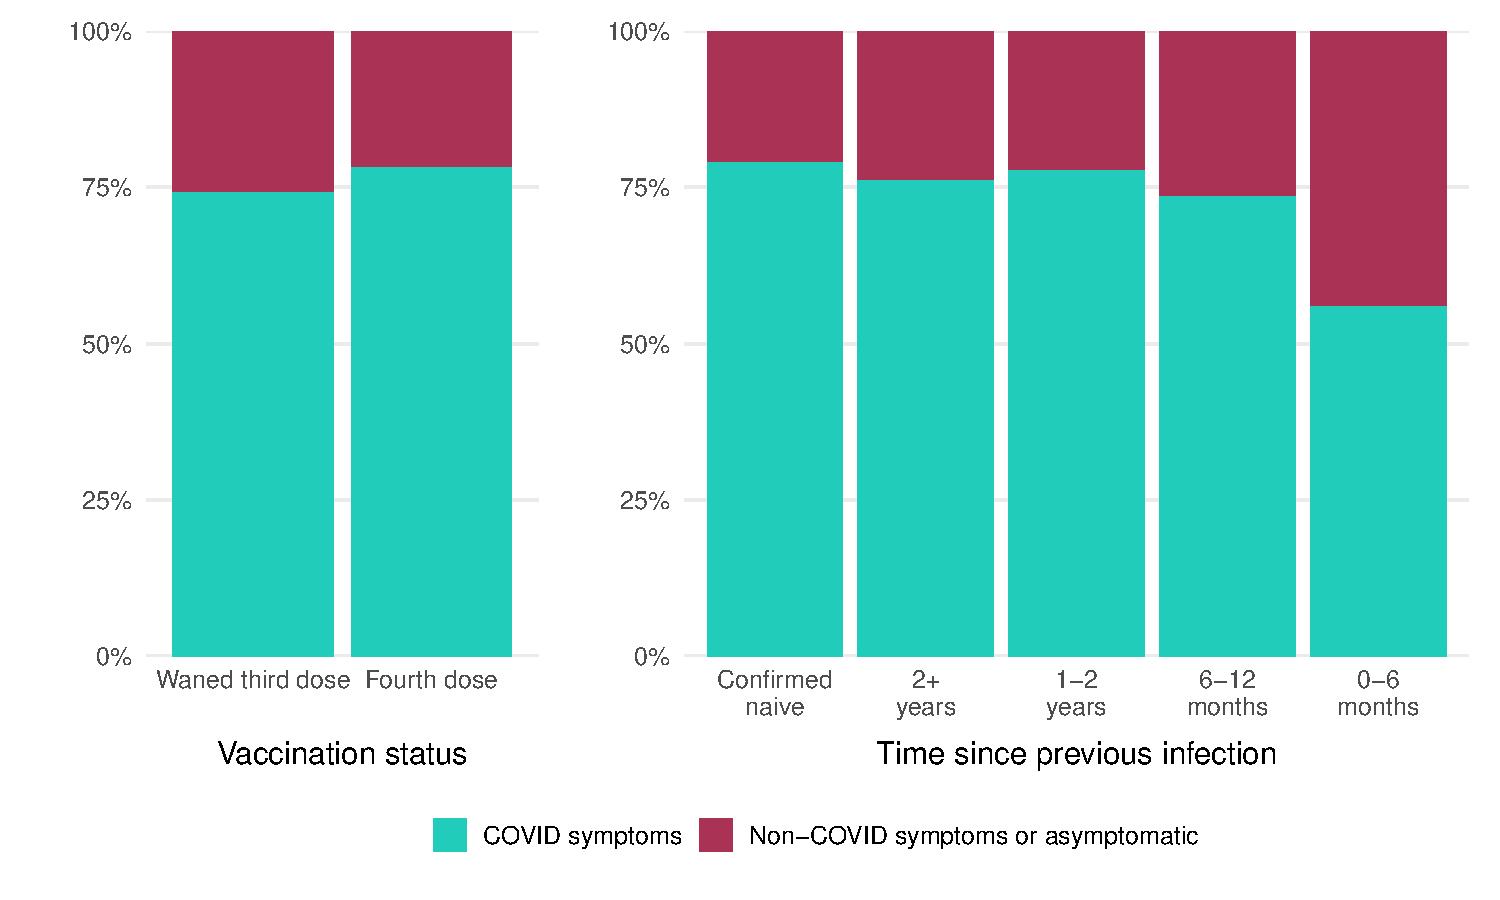
\includegraphics[width=\textwidth]{symptoms_vaccine_tsp.pdf}
    \caption[Self-reported symptom status among SIREN participants testing positive for COVID-19, by vaccination status, and time since previous infection]{Self-reported symptom status among SIREN participants testing positive for COVID-19, by vaccination status (panel A), and time since previous infection (panel B).}\label{fig:symptoms_vaccine_tsp}
\end{figure}

\subsubsection{Vaccine effectiveness}

Vaccine effectiveness of the fourth (booster) dose relative to protection at least six-months after a third dose was estimated as 13.1\% (95\% CI 0.9 to 23.8\%) over the entire analysis period (Figure~\ref{fig:ve_long} panel A). VE was highest in the two months post-vaccination at 24.0\% (95\% CI 8.5 to 36.8\%), reducing to 10.3\% (95\% CI -11.4 to 27.8\%) in the period two-to-four months post-vaccination, and 1.7\% (95\% CI -17.0 to 17.4\%) in the period four-to-six months post-vaccination (Figure~\ref{fig:ve_long} panel B). Relative to a waned third dose, VE was 8.6\% (95\% CI -5.8 to 20.9\%) against symptomatic infection and 28.0\% (95\% CI 6.6 to 44.5\%) against asymptomatic infection (Figure~\ref{fig:ve_long} panel D and E).

SARS-CoV-2 infection within the last 6 months was associated with a 63.6\% (95\% CI 46.8 to 75.0\%) increase in protection compared to individuals who had an infection more than 2 years ago (Figure~\ref{fig:ve_long} panel C). This protection was 72.0\% (95\% CI 56.1 to 82.1) against symptomatic infection and 42.2\% (95\% CI -17.8 to 72.7) against asymptomatic infection (Figure~\ref{fig:ve_long} panel F). Corresponding estimates with the confirmed na\"{\i}ve group used as the baseline are shown in Figure~\ref{fig:ve_baseline}. Table~\ref{tab:pcr_positivity} includes these estimates alongside crude PCR positivity rates (number of detected PCR positive results per 10,000 person-days of follow-up).

\begin{figure}[htbp!]
    \centering
    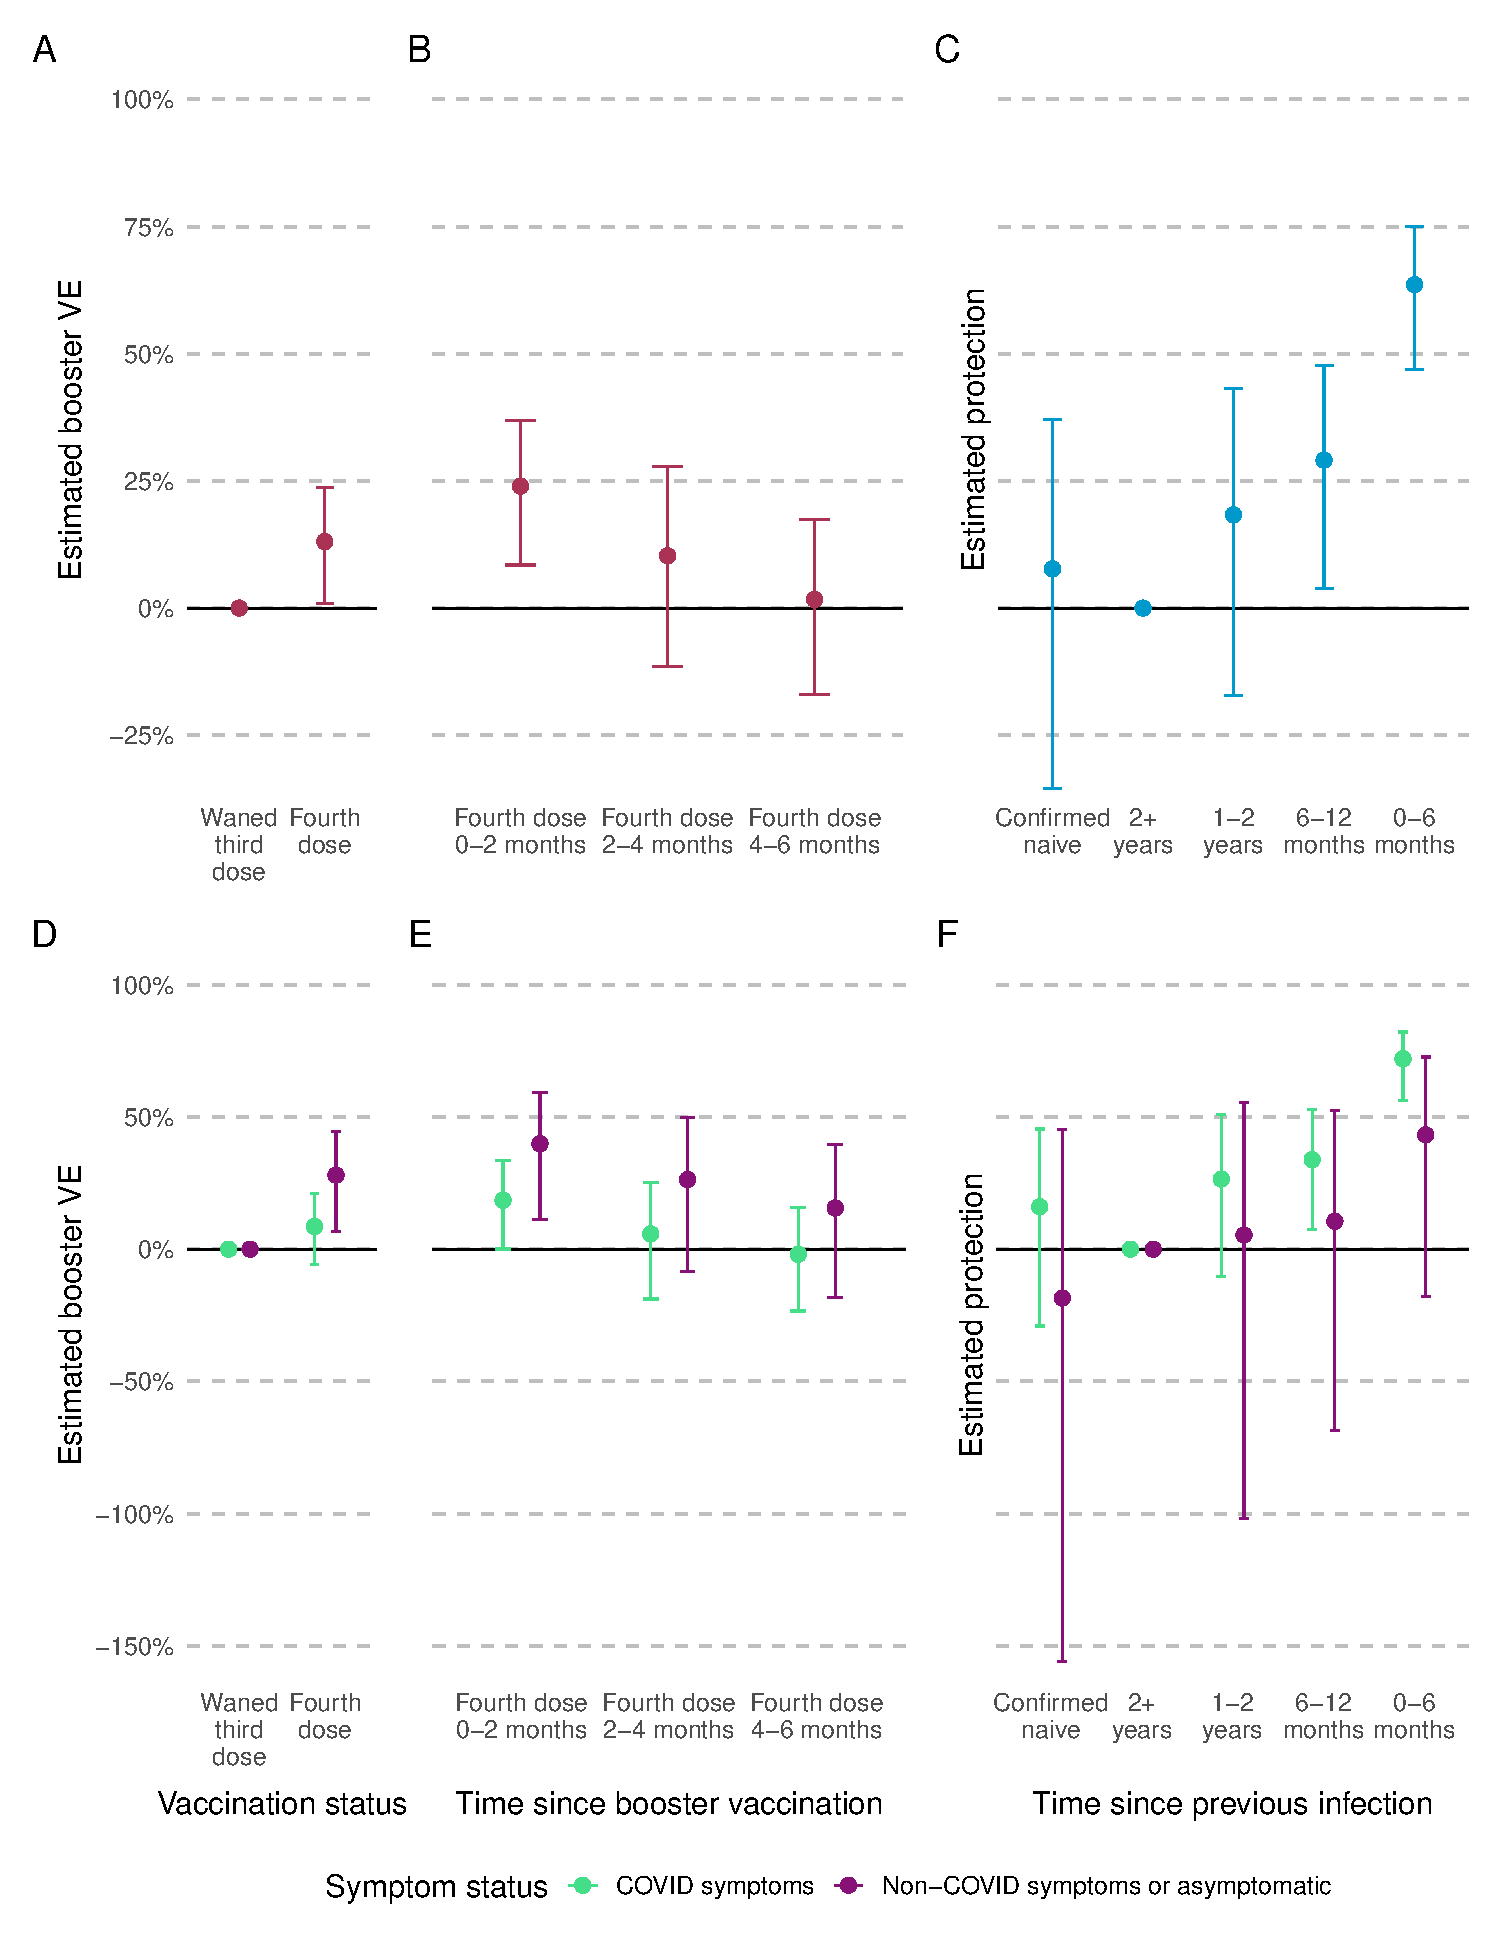
\includegraphics[width=\textwidth]{ve_long.pdf}
    \caption[Estimated booster VE by booster vaccination status, time since booster vaccination, and estimated protection from previous infection]{Estimated booster VE by booster vaccination status (panel A, model M1), time since booster vaccination (panel B, model M2), and estimated protection from previous infection (panel C, model M3), and symptom status (panels D--F, models M5--M7). Error bars show the 95\% CI around the estimates.}\label{fig:ve_long}
\end{figure}

\subsubsection{Mean sojourn time in PCR positive state}

The mean sojourn time in the PCR positive state was estimated as 7.5 days (95\% CI 6.9 to 8.1) overall (Figure~\ref{fig:sojourn-time} panel A). When averaged over the study population, the mean sojourn time was 6.9 days (95\% CI 5.9 to 8.1) among those with a booster vaccination, compared to 8.5 days (95\% CI 6.8 to 10.6) for those with a waned third dose (Figure~\ref{fig:sojourn-time} panel B).

The mean sojourn time was 9.5 days (95\% CI 7.1 to 12.8) for confirmed na\"{\i}ve participants and 7.3 days (95\% CI 6.3 to 8.3) for those with an infection within the past 0--6 months (Figure~\ref{fig:sojourn-time} panel C). Infections reported as symptomatic had a mean sojourn time of 8.1 days (95\% CI 7.4 to 8.9), compared to 4.7 days (95\% CI 4.0 to 5.5) for asymptomatic (Figure~\ref{fig:sojourn-time} panel D). 

\begin{figure}[htbp!]
    \centering
    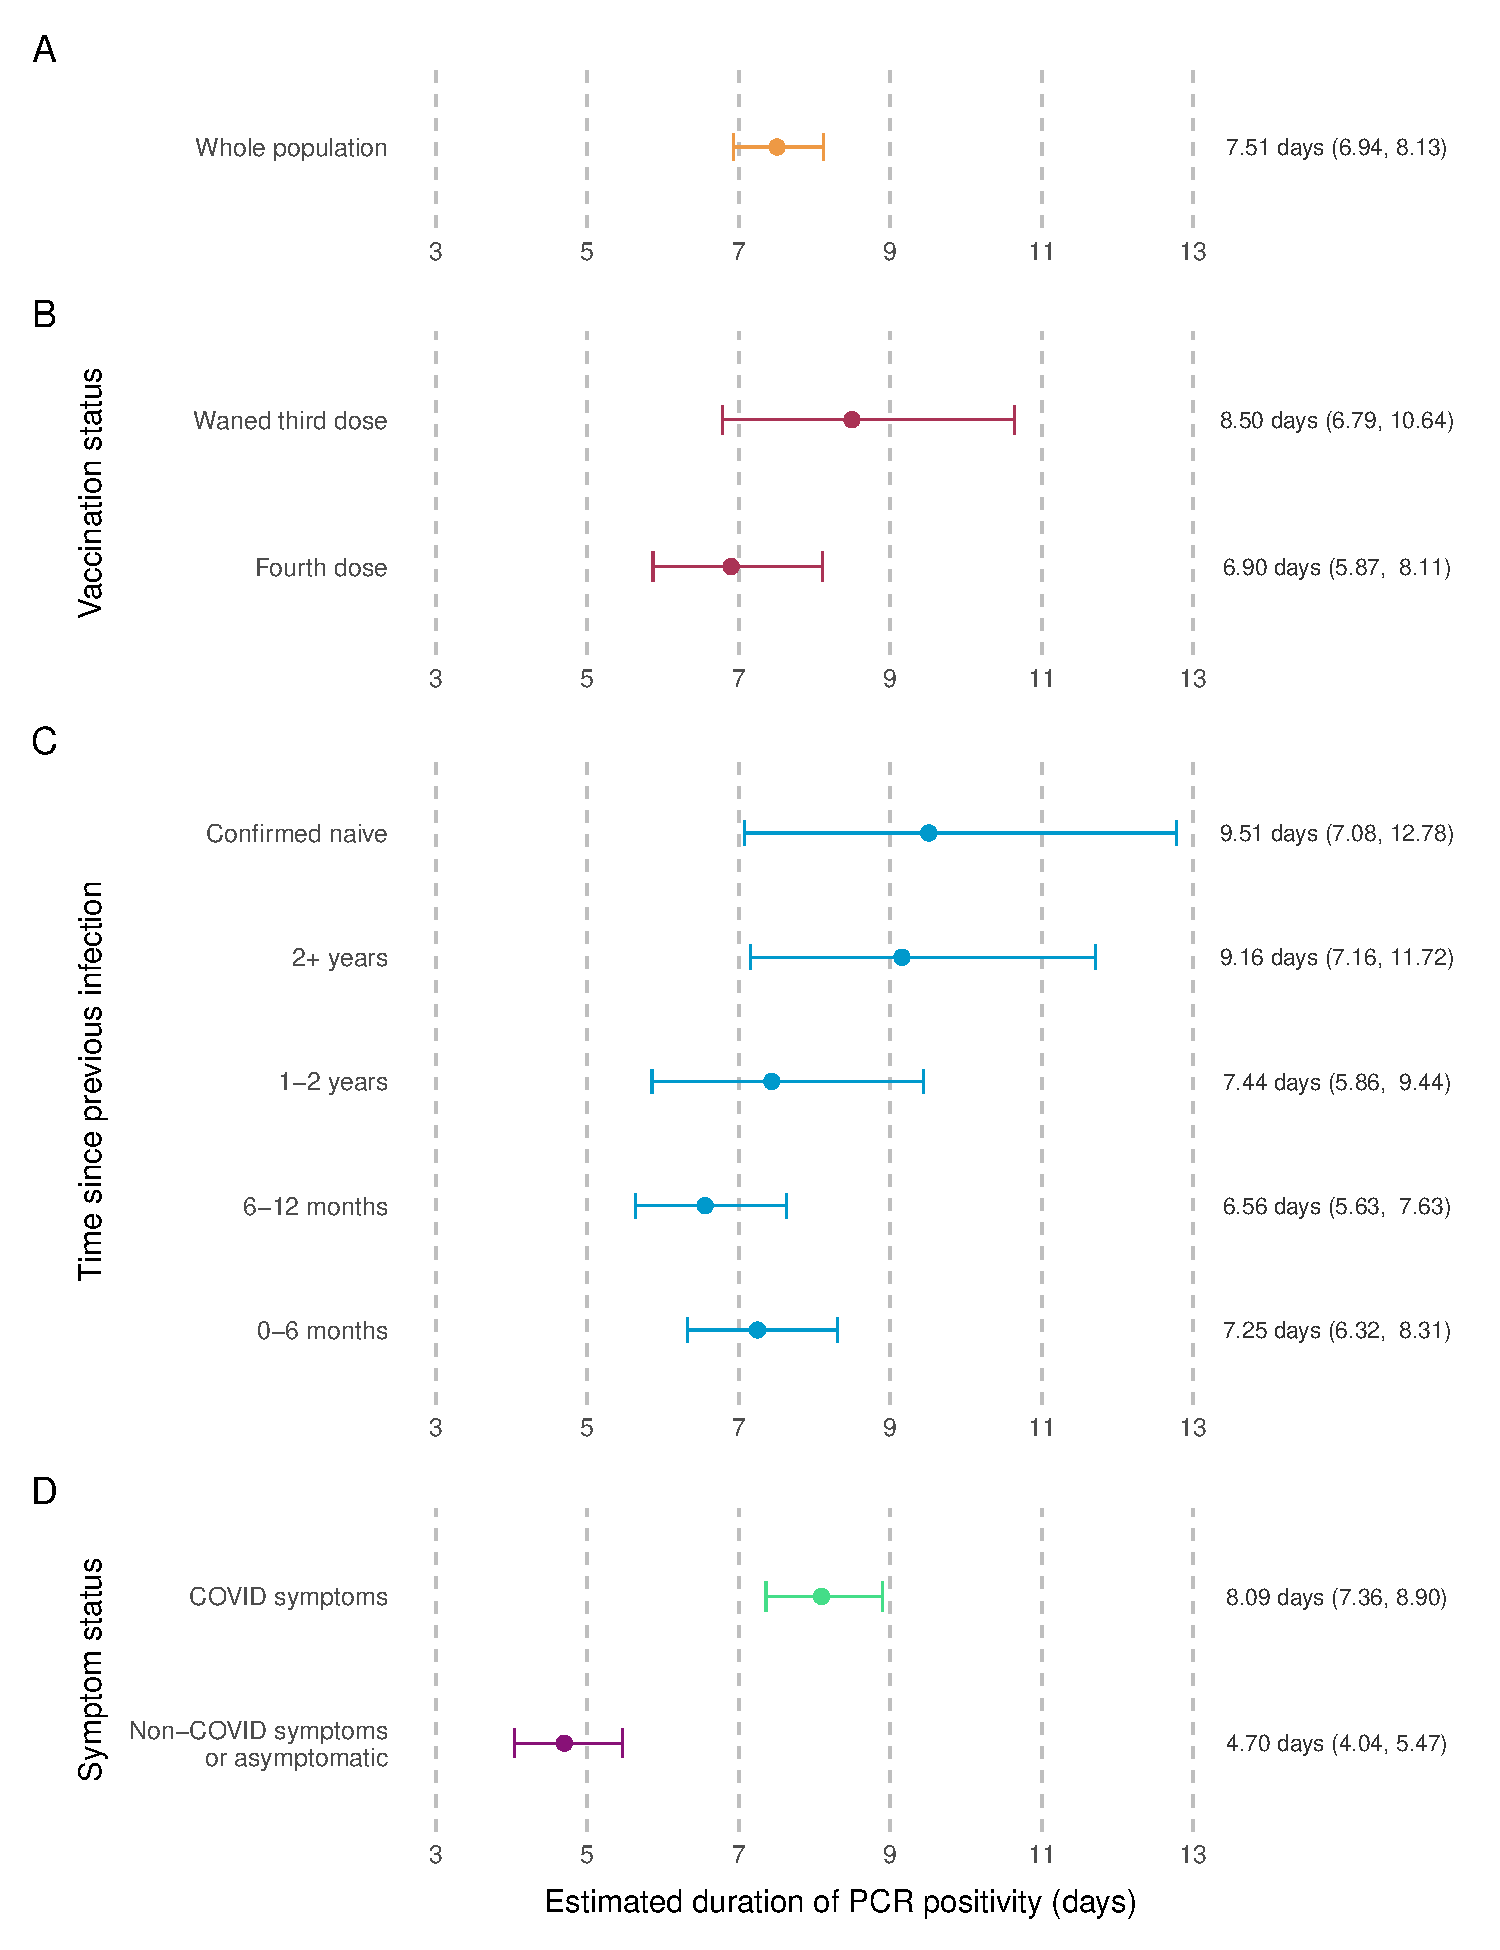
\includegraphics[width=\textwidth]{sojourn_time.pdf}
    \caption[Estimated mean sojourn time in PCR positive state, averaged across the study population, by vaccination status, time since previous infection, and symptom status]{Estimated mean sojourn time in PCR positive state, averaged across the study population, overall (panel A, model M1), by vaccination status (panel B, model M1), time since previous infection (panel C, model M2), and symptom status (panel D, model M5). Error bars show the 95\% CI around the estimates.}\label{fig:sojourn-time}
\end{figure}

Table~\ref{tab:sojourn_time} includes the mean sojourn time estimates alongside empirical estimates of the duration of PCR positivity, calculated as the median time from initial PCR positive to subsequent PCR negative.

\subsubsection{Goodness of fit}

A comparison between the forecast number of individuals occupying the infected state and the more empirical estimate derived from the observed data was used to assess model fit. For the two-state model, the empirical estimate was within the confidence intervals of the fitted model throughout most of the study period, but fell below the lower 95\% CI of forecast prevalence in weeks 12--16 (Figure~\ref{fig:model_diagnostics}).

\begin{figure}[htbp!]
    \centering
    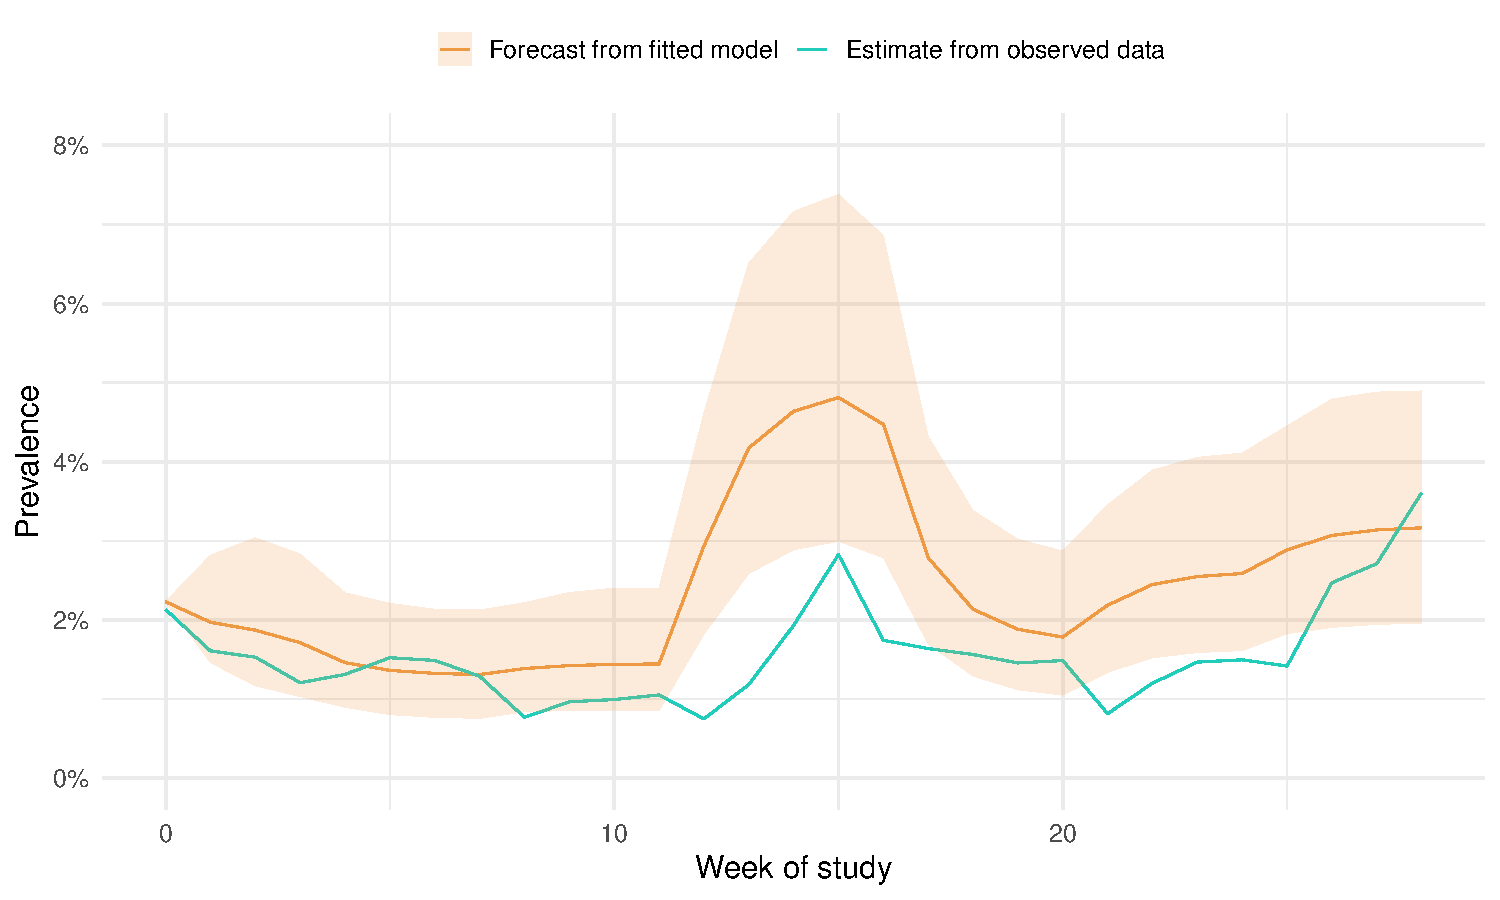
\includegraphics[width=\textwidth]{model_diagnostics.pdf}
    \caption[Comparison of prevalence in the infected state forecast from fitted model and more empirical estimate over time]{Comparison of prevalence in the infected state forecast from fitted model M1 and more empirical estimate over time. Shaded area shows the 95\% CI around the expected prevalence.}\label{fig:model_diagnostics}
\end{figure}

Table~\ref{tab:siren_deviance} shows the deviance test statistic for the two-state model fitted to the SIREN data. Time intervals 1 and 2 represent more and less frequent testers, respectively. Covariate categories A and B represent are partitions of the data based on quantiles of the estimated transition intensities $q_{r,s}$~\parencite{Titman2009-nk}. The test statistic varied most according to time interval, with the greatest deviance among less frequent testers (time interval 2) and for the susceptible to infection transition.

\begin{table}[!h]
\centering
\caption{\label{tab:siren_deviance}Deviance statistics for fitted multi-state model M1, by time from study start, time interval, and covariate strata.}
\centering
\begin{tabular}[t]{lllrr}
\toprule
\makecell[l]{Time from study\\start (weeks)} & \makecell[l]{Time\\interval} & \makecell[l]{Covariate\\category} & \makecell[l]{Susceptible to\\infected transition} & \makecell[l]{Infected to\\susceptible transition}\\
\midrule
\cellcolor{gray!10}{{}[0.14,16.29)} & \cellcolor{gray!10}{1} & \cellcolor{gray!10}{A} & \cellcolor{gray!10}{5.71} & \cellcolor{gray!10}{-5.46}\\
{}[16.29,28.57] & 1 & A & 7.11 & -0.37\\
\cellcolor{gray!10}{{}[0.14,16.29)} & \cellcolor{gray!10}{2} & \cellcolor{gray!10}{A} & \cellcolor{gray!10}{-18.39} & \cellcolor{gray!10}{-0.01}\\
{}[16.29,28.57] & 2 & A & -25.59 & 0.02\\
\cellcolor{gray!10}{{}[0.14,16.29)} & \cellcolor{gray!10}{1} & \cellcolor{gray!10}{B} & \cellcolor{gray!10}{0.04} & \cellcolor{gray!10}{-6.53}\\
{}[16.29,28.57] & 1 & B & 0.04 & -2.30\\
\cellcolor{gray!10}{{}[0.14,16.29)} & \cellcolor{gray!10}{2} & \cellcolor{gray!10}{B} & \cellcolor{gray!10}{0.49} & \cellcolor{gray!10}{-0.64}\\
{}[16.29,28.57] & 2 & B & 0.00 & -0.28\\
\bottomrule
\end{tabular}
\end{table}


Lastly, Appendix~\ref{appendix:siren-gof} shows the expected number of infections simulated under different sampling schemes, for instance all participants testing on a bi-weekly basis.

\subsubsection{Comparison of model estimates}

The Cox proportional hazards model is equivalent to a two-state model without recovery or interval censoring. Figure~\ref{fig:vaccine_short} compares the hazards estimated in multi-state model M1 to those from the corresponding stratified Cox proportional hazards model, where the same covariates are included in both models. Point estimates were very similar between the two models, with estimates from the multi-state model having slightly wider confidence intervals. Additional comparisons are included in Figures~\ref{fig:vaccine_long} and~\ref{fig:vaccine_short_noev}.

\begin{figure}[htbp!]
    \centering
    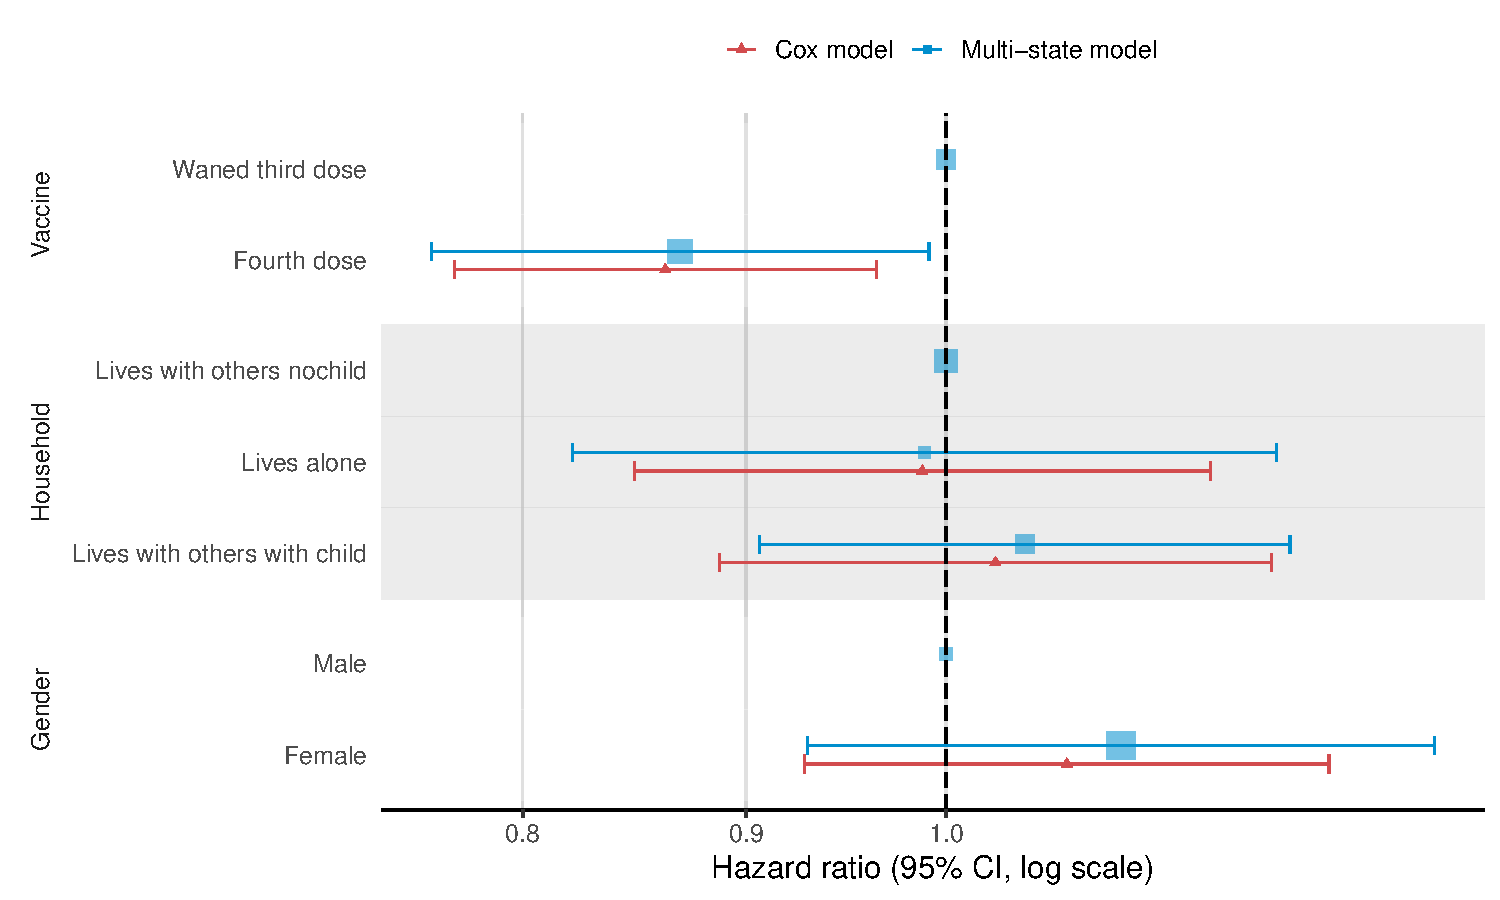
\includegraphics[width=\textwidth]{vaccine_short.pdf}
    \caption[Comparison of hazards estimated by multi-state and Cox proportional hazards model]{Comparison of hazards estimated by multi-state model M1 and the corresponding Cox proportional hazards model, for covariates common between the two models. Error bars show the 95\% CI around the estimated hazards.}\label{fig:vaccine_short}
\end{figure}

\subsection{Discussion}

Multi-state models were successfully applied to the SIREN data to jointly estimate the effectiveness of fourth dose mRNA vaccines against infection and the mean sojourn time in the PCR positive state over the period September 2022 to March 2023. Models were applied in real-time throughout the study period, with interim estimates presented to UKHSA and the JCVI to inform booster vaccination policy~\parencite{Department-of-Health-and-Social-Care2023-um}.

Controlling for prior infection, fourth dose mRNA vaccine effectiveness against infection was estimated around 24\% in the first 2 months post-vaccination, with significant waning of protection thereafter. These estimates are in-line with bivalent booster vaccine effectiveness estimates among healthcare workers in the US~\parencite{Shrestha2023-oq}, and corroborate the results of other cohort studies~\parencite{Auvigne2023-ay, Huiberts2023-kq}.

Mean duration of PCR positivity estimates were also consistent with previous studies, most of which have estimated a mean duration of positivity for Omicron-era infections of around 7 days~\parencite{Hay2022-sg, UK_Health_Security_Agency2023-us, Boucau2022-it, Pei2023-qd, Kojima2022-vh}. The estimates from the multi-state model uncover additional distinctions between sub-groups which are missed by an empirical approach and have not been previously reported, such as mean duration of PCR positivity by symptom status.

The divergence in infection prevalence estimated by the observed data and forecast from the fitted multi-state model coincided with the December and new year period, when lower adherence to the fortnightly testing schedule was seen in the data. This highlights the utility of the multi-state model, which is able to account for potentially unobserved infections in intermittently observed data. With optimal fortnightly testing it is likely that a greater number of infections would have been detected. Future analyses of the this cohort will use multi-state models to account for intermittent observation, thereby reducing biases from sub-optimal sampling.

Similar hazard ratio estimates were obtained from the multi-state and Cox proportional hazards models. The slightly wider confidence intervals in the multi-state model estimates may be a more accurate reflection of their uncertainty, given that they account for intermittent observation and missed testing. 

Additional results from this analysis are available in the published manuscript and supplementary materials~\parencite{Kirwan2024-hj}.

\subsection{Limitations}\label{sec:siren-limitations}

Whilst this cohort analysis addressed specific biases of test-negative case-control studies, as described in Section~\ref{sec:cohort-study-design}, certain limitations remain. Firstly, while piecewise-constant hazards were used to account for non-proportionality, the proportional hazards assumption may still be unrealistic for the covariates we have studied. Non-proportional hazards are common in medical studies, and~\cite{Stensrud2020-wa} have recommended interpreting modelled hazard ratios as a weighted average of the true hazard ratios over the entire follow-up period.

Secondly, the Markov assumption was unlikely to hold true immediately post-infection or immediately post-recovery, although the extent of this issue is likely to be small in comparison to the long follow-up time. As shown in Appendix~\ref{appendix:alt-models}, the convalescent model did not provide significantly different hazards estimates, perhaps as the time since previous infection covariate already accounts for some of this variability. The semi-Markov model relaxes the Markov assumption but this model exhibited identifiability issues and was sensitive to initial values, likely a result of insufficient data on infections.

Another potential limitation of the chosen models was the assumption of no state misclassification. The Coronavirus Infection Survey (CIS) has previously estimated PCR test sensitivity of between 85--98\%~\parencite{Wei2023-ry}. Results from the misclassification model with fixed misclassification probabilities are included in Appendix~\ref{appendix:alt-models}; estimated booster VE and protection from prior infection were similar to estimates from the two-state model without misclassification. As the SIREN study includes both serial PCR and linked antibody testing data, and allows for manual review in case of inconsistent results, the extent of misclassification in this cohort was expected to be small.

Lastly, non-informative sampling is an assumption of the model. The presence of informative sampling would lead to an overestimate of the probability of detecting infection, e.g.\ if participants choose to test because of symptoms. For this study the majority of SIREN study participants did test according to the fortnightly schedule (albeit with reduced frequency during December), and only a small degree of out-of-schedule PCR testing was observed.

\section{Causal effect of vaccination}\label{sec:siren-causal}

So far this chapter has investigated the effects associated with an intervention, specifically vaccination, using observational data. Commonly of greater interest, however, are the causal effects of such an intervention. By explicitly stating the causal assumptions and controlling for confounding and selection bias, causal inference methods allow findings from observational studies to be interpreted in a causal way~\parencite{Ryalen2020-nl, Hernan2006-ei}.

Causal inference methods have been applied in several COVID-19 vaccine effectiveness studies to estimate the causal effect of vaccination at different stages in the pandemic~\parencite{Dagan2021-ow, Xie2022-np, Hulme2023-fw}. In this section I specify a causal inference method and the necessary assumptions for making causal statements using continuous-time multi-state models. This method is applied to the SIREN data to estimate the causal effect of vaccination in this cohort.

\subsection{Artificial manipulation of transition intensities}

Artificial manipulation of transition intensities (AMTI)\nomenclature[z]{AMTI}{Artificial manipulation of transition intensities} is a method of causal inference for continuous-time multi-state models. AMTI has been used to investigate counterfactual scenarios in multi-state models, for example the effect of a hypothetical change in sickness benefits on absence, and the effect of hypothetical treatment regimes for transplant patients~\parencite{Keiding2001-lk, Gran2015-fc}.

AMTI involves intervening on specific entries of an estimated transition intensity matrix, $\mathbf{Q}$. These entries may be fixed to particular values which represent a hypothetical intervention, for instance complete vaccination of a cohort. The intervened-upon transition intensity matrix is $\mathbf{{\tilde{Q}}}$ and quantities of interest can be estimated from the corresponding transition probability matrix, $\mathbf{{\tilde{P}}}$.

Before deriving causal estimates using AMTI, I will firstly explicitly state the required causal assumptions. The causal assumptions for a continuous-time parametric proportional hazards model with piecewise-constant baseline hazards are a special case of those formalised by~\cite{Ryalen2020-nl} to infer the causal effect of treatment on survival for cancer patients.

\subsubsection{Local independence graphs}

A local independence graph which represents short-term causal relationships between continuous processes in the SIREN study is shown in Figure~\ref{fig:siren-local-independence-graph}. Here A represents vaccination, Z are confounders (e.g.\ age, occupation, prior infection), and Y represents infection. The local independence graph represents the assumptions that vaccination has a causal relationship with infection, and that the confounders (baseline covariates) have a causal relationship with both vaccination and infection.

\begin{figure}[htbp!]
    \centering
    \begin{tikzpicture}
        % x node set with absolute coordinates
        \node (a) at (0,0) {$Z$};
        \node (b) [below =of a] {$A$};
        \node (c) [right =of a] {$Y$};

        % Directed edge
        \path (a) edge[bend right = 20] (b);
        \path (a) edge[bend left = 20] (c);
        \path (b) edge[bend right = 20] (c);

    \end{tikzpicture}
    \caption[Local independence graph with A representing vaccination, Z representing confounders, and Y representing infection]{Local independence graph with A representing vaccination, Z representing confounders, and Y representing infection.}\label{fig:siren-local-independence-graph}
\end{figure}

\subsubsection{Participant information}

Participants in the study are assumed to be i.i.d.\ over the study period $[0, \tau]$. For each participant, $i$, with baseline covariates $Z_i$, define a set of counting processes~\parencite{Aalen2008-rf}:
%
\begin{itemize}
    \item $\left(N_i^I(t) : t \geq 0\right)$ the counting process for entries into the infected state by time $t \geq 0$, i.e.\ $N_i^I(t)$ is the number of times the participant has entered the infection state by time $t$;
    \item $\left(N_i^S(t) : t \geq 0 \right)$ the counting process for returning to the susceptible state by time $t \geq 0$;
    \item $\left(A_i(t) : t \geq 0 \right)$ the counting process for vaccination at time $t \geq 0$, i.e.\ $A_i(t) = 1$ if the participant has been vaccinated by time $t$, and $A_i(t) = 0$ otherwise.
\end{itemize}

Henceforth the $i$ notation will be omitted for brevity, i.e.\ $N^I(t) \equiv N_i^I(t)$, $Z \equiv Z_i$, and $A(t) \equiv A_i(t)$.

Let
%
\begin{align*}
    \bar{N}^I(t) & = \{N^I(s): s \leq t \} \\
    \bar{N}^S(t) & = \{N^S(s): s \leq t \} \\
    \bar{A}(t)   & = \{A(s): s \leq t \}
\end{align*}

represent the history of each counting process up to time $t$. Define the vaccination status for an individual at the end of the study period as $\bar{A} = \bar{A}(\tau)$, and let $N^{I,\bar{a}}(t)$ and $N^{S,\bar{a}}(t)$ be the counting processes at time $t$ when we intervene to set $\bar{A} = \bar{a}$, i.e.\ the number of times the participant would have entered the infected state/returned to the susceptible state by time $t$ when we intervene to set $\bar{A} = \bar{a}$.

Let $q^I(t)$ be the transition intensity at time $t$ for counting process $N^I(t)$:
%
\begin{align*}
     & q^I(t \mid Z, \bar{A} (t \mbox{-}), \bar{N}^I (t \mbox{-}), \bar{N}^S (t \mbox{-}))                                                                                    \\
     & = \lim_{\delta t \downarrow 0} \left\{\frac{\Pr\left(N^{I}(t) - N^{I}(t - \delta t) > 0 \mid Z, \bar{A} (t - \delta t), \bar{N}^I (t - \delta t), \bar{N}^S (t - \delta t)\right)}{\delta t}\right\}
\end{align*}

where $t\mbox{-}$ represents the instant before time $t$. The transition intensities for counting processes $N^S(t)$, $N^{I,\bar{a}}(t)$ and $N^{S,\bar{a}}(t)$ are, respectively:
%
\begin{align*}
     & q^S(t \mid Z, \bar{A} (t \mbox{-}), \bar{N}^I (t \mbox{-}), \bar{N}^S (t \mbox{-}))            \\
     & q^{I, \bar{a}}(t \mid Z, \bar{N}^{I, \bar{a}} (t \mbox{-}), \bar{N}^{S, \bar{a}} (t \mbox{-})) \\
     & q^{S, \bar{a}}(t \mid Z, \bar{N}^{I, \bar{a}} (t \mbox{-}), \bar{N}^{S, \bar{a}} (t \mbox{-}))
\end{align*}

\subsubsection{Causal assumptions}

Suppose that we make a hypothetical, but meaningful, intervention on a transition intensity $q^{I}$ to set $\bar{A} = \bar{a}$, then under the assumption of `local independence' this intervention will not change the `local' characteristics for other transition intensities and covariate effects~\parencite{Seaman2023-rs, Ryalen2019-it}:
%
\begin{align*}
     & q^I (t \mid Z = z, \bar{A} (t \mbox{-}) = \bar{a} (t \mbox{-}), \bar{N}^I (t \mbox{-}) = \bar{n}^I (t \mbox{-}), \bar{N}^S (t \mbox{-}) = \bar{n}^S (t \mbox{-})) \\
     & = q^{I, \bar{a}} (t \mid Z = z, \bar{N}^{I, \bar{a}} (t \mbox{-}) = \bar{n}^I (t \mbox{-}), \bar{N}^{S, \bar{a}} (t \mbox{-}) = \bar{n}^S (t \mbox{-}))
\end{align*}

and, analogously, for $q^{S}$:
%
\begin{align*}
     & q^S (t \mid Z = z, \bar{A} (t \mbox{-}) = \bar{a} (t \mbox{-}), \bar{N}^I (t \mbox{-}) = \bar{n}^I (t \mbox{-}), \bar{N}^S (t \mbox{-}) = \bar{n}^S (t \mbox{-})) \\
     & = q^{S, \bar{a}} (t \mid Z = z, \bar{N}^{I, \bar{a}} (t \mbox{-}) = \bar{n}^I (t \mbox{-}), \bar{N}^{S, \bar{a}} (t \mbox{-}) = \bar{n}^S (t \mbox{-}))
\end{align*}

for all possible values $z \in Z$, $\bar{a} (t \mbox{-}) \in \bar{A}(t\mbox{-})$, $\bar{n}^I (t \mbox{-}) \in \bar{N}^I (t \mbox{-})$, and $\bar{n}^S (t \mbox{-}) \in \bar{N}^S (t \mbox{-})$.

Now make the simplifying assumption that the transition intensities only depend on the binary indicator of vaccination, and not on the history of the vaccination process:
%
\begin{align*}
    q^I (t \mid Z, \bar{A} (t \mbox{-}), \bar{N}^I (t \mbox{-}), \bar{N}^S (t \mbox{-})) & =
    q^I (t \mid Z, A(t \mbox{-}), \bar{N}^I (t \mbox{-}), \bar{N}^S (t \mbox{-}))            \\
    q^S (t \mid Z, \bar{A} (t \mbox{-}), \bar{N}^I (t \mbox{-}), \bar{N}^S (t \mbox{-})) & =
    q^S (t \mid Z, A(t \mbox{-}), \bar{N}^I (t \mbox{-}), \bar{N}^S (t \mbox{-}))
\end{align*}

`Consistency' and `no interference' is also assumed (known as the Stable Unit Treatment Value Assumption (SUTVA)\nomenclature[z]{SUTVA}{Stable unit treatment value assumption}). By SUTVA, there are no other forms of treatment, i.e.\ $N^I(t) = N^{I, \bar{a}}(t)$ for individuals with $\bar{A}(t\mbox{-}) = \bar{a}(t\mbox{-})$, and a participant's outcomes do not depend on whether or not other participants were vaccinated~\parencite{VanderWeele2013-iw}.

Lastly, parametric models are assumed for $q^I$ and $q^S$, with proportional hazards and a piecewise-constant baseline hazard.

\subsection{Application to SIREN}

An intervention to set $\left(A(t) = a(t): t \geq 0\right)$ corresponds to either all participants receiving a fourth vaccine booster dose at time $t$ or none receiving a booster dose. To investigate the causal effect of vaccination in this cohort, two specific interventions were considered:
%
\begin{enumerate}
    \item[A.] \textbf{No vaccination}:\ all participants begin in the susceptible state and no vaccination is received, corresponding to $a(t) = 0$ for all $t \geq 0$;
    \item[B.] \textbf{Complete vaccination at time zero}:\ all participants begin in the susceptible state and receive a vaccine booster at the start of the study, corresponding to $a(t) = 1$ for all $t \geq 0$.
\end{enumerate}

\subsubsection{Estimation procedure}

Let $N^{I,a}_{\text{TOT}}$ be the total number of infections across all individuals and the whole study period, $[0, \tau]$, when we set $A(t) = a(t)$. The expected number of infections under each hypothetical scenario is then defined as:
%
\[
    \mathbb{E}\left(N^{I,a}_{\text{TOT}}; q^{I, a}\right) = \sum_i \left\{ \int_{t = 0}^\tau q^{I, a}(t \mid Z_i, \bar{N}_i^{I, a} (t \mbox{-}), \bar{N}_i^{S, a} (t \mbox{-})) \dif t \right\}
\]

Since, in practice, $q^{I,a}$ is unknown, artificial manipulation of transition intensities (AMTI) is applied to the maximum likelihood estimate $\hat{q}^I$ that was obtained from the fitted model to estimate $\mathbb{E}(N^{I,a}_{\text{TOT}}; \hat{q}^{I,a})$, which corresponds to the intervention $A(t) = a(t)$.

Confidence intervals may be calculated by drawing a a random sample from the multivariate normal distribution with mean $\hat{q}$ and covariance matrix as estimated using the maximum likelihood estimator (by the asymptotic normality of this estimator~\parencite{Young2005-vx}) and taking the 2.5 and 97.5 percentiles.

The causal effect of vaccination was calculated by comparing the total number of expected infections under the `no vaccination' and `complete vaccination' counterfactual scenarios. For this study, the cohort was assumed to remain under follow-up for the whole study period, so that all infections (regardless of whether they would have been detected) were counted.

\subsubsection{Covariates}

For a causal analysis, all relevant confounders which could be causal to both an individual in the study choosing to be vaccinated and becoming infected should be included as covariates, whilst not conditioning on common effects of vaccination and infection. Time-varying covariates (i.e.\ $Z(t)$) may be included provided there is no time-varying confounding~\parencite{Ryalen2020-nl}.

Comparable COVID-19 vaccine trial emulation studies have included similar covariates to the association study described in Section~\ref{sec:siren-msm} (calendar month, vaccination history, time since previous infection, age group, gender, and region)~\parencite{Xie2022-np, Hulme2023-fw, Barda2021-dq}. Two studies set in the UK additionally included clinical risk group and index of multiple deprivation (IMD) in their analyses~\parencite{Xie2022-np, Hulme2023-fw}. Whilst these covariates were available they were not chosen for the association study as the IMD measure was unavailable for certain regions and as conditioning on clinical risk group did not improve model fit.

To capture potential infection risk among this cohort, both within and outside of the clinical workplace setting, the covariates considered in the causal model were:\ calendar month, vaccination history, time since infection, age group, gender, region, clinical risk group, IMD, occupation/setting, household status, and patient contact.  Calendar month and time since infection were allowed to be time-varying with the time since infection covariate only relating to infections acquired prior to study start.

For the hypothetical scenarios described:\ the vaccination covariate was fixed to the specified intervention value; the calendar month covariate was included and changed linearly with time; the time since prior infection covariate was specified to relate only to infections prior to the study and increased linearly with time; all other covariates were fixed to the values they were observed as in the data.

\subsection{Results}

The expanded model, including clinical risk group and index of multiple deprivation, was fitted to a subset of the data with complete information for all covariates. This subset included 6553 participants, among whom 1023 infections were detected. A comparison between the forecast number of individuals occupying the infected state and an estimate derived from the observed data was used to assess model fit for the expanded model, included in Appendix~\ref{appendix:siren-gof}.

Figure~\ref{fig:passage-probs} shows the estimated number of infections under each counterfactual scenario. The expected number of infections when no participants received vaccination was 3101 (95\% CI 2326 to 3981), and the expected number of infections when all participants received vaccination at time zero was 2660 (95\% CI 1992 to 3477). The causal effect of fourth dose vaccination for this cohort was therefore 441 averted infections, albeit with substantial overlap of confidence intervals.

\begin{figure}[htbp!]
    \centering
    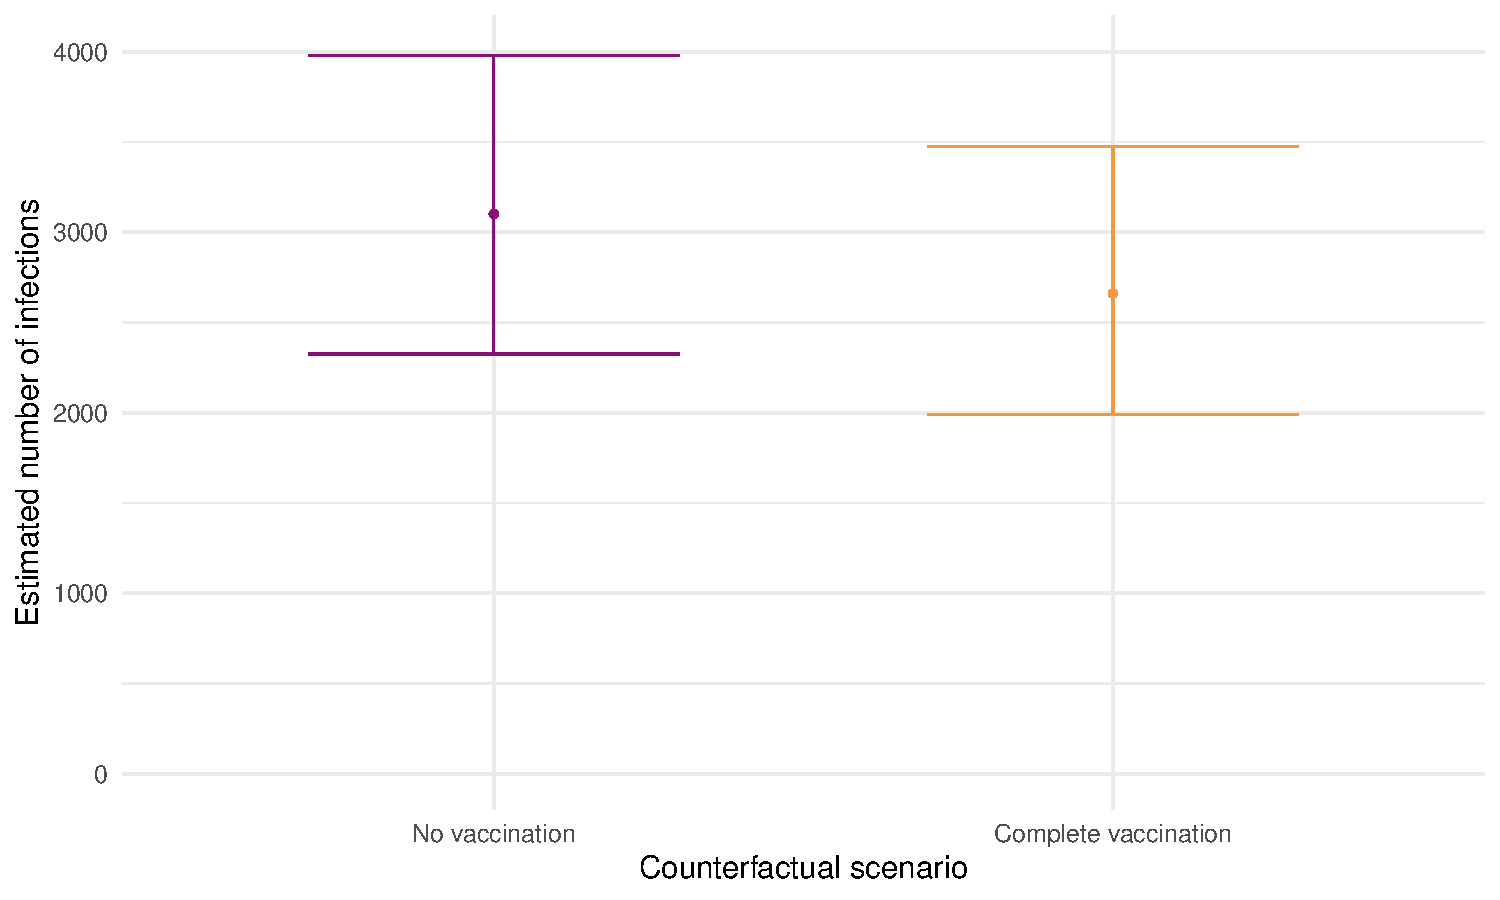
\includegraphics[width=\textwidth]{ppass_causal_msm.pdf}
    \caption[Estimated total number of infections under the `No vaccination' and `Complete vaccination' counterfactual scenarios]{Estimated total number of infections under the `No vaccination' and `Complete vaccination' counterfactual scenarios.}\label{fig:passage-probs}
\end{figure}

\subsection{Discussion}

In this analysis I have estimated the causal effect of vaccination upon SARS-CoV-2 infection among SIREN study participants by comparing the total number of expected infections under two counterfactual scenarios.

The proportion of infections estimated to have been averted through vaccination was relatively small (around 14\%), with overlapping confidence intervals due to the uncertainty in the parameter estimates. The counterfactual estimates reflect the total number of infections in each hypothetical cohort over the entire time period, regardless of whether or not the infection would be detected. The detected number of infections in the association study was significantly lower than in this causal analysis ($n = 1023$), both because the data in the association study were intermittently observed, and as participants may have dropped-out of follow-up.

Despite a modest number of averted infections, there are accompanying causal effects of vaccination which may also reduce the burden of infection in this cohort. The mean duration of PCR positivity was estimated to be reduced among those who were vaccinated, which may result in a reduction in sick leave. Other metrics, including cost and impact on patient infections, have previously been used to investigate the utility of SARS-CoV-2 interventions~\parencite{Heath2023-af} and vaccination may mitigate adverse events such as hospital admission, as discussed in Chapter~\ref{cha:hospitalseverity}. These metrics could provide a wider understanding of the causal effects of vaccination, if sufficient data were available.

\subsubsection{Limitations}

The same potential biases of informative sampling and state misclassification discussed in Section~\ref{sec:siren-limitations} are present in this analysis but, as before, the effects from these biases are likely to be small.

Neither the i.i.d.\ assumption, nor the assumption of no interference are credible for this study (or infectious disease studies in general):\ healthcare workers may well transmit infection between themselves, and there may well be `spillover' effects of one individual's vaccination on another individual's infection risk. Clustering data at hospital-level, rather than individual-level, could account for this interference, but this would reduce the sample size considerably and means individual-level confounders cannot be accounted for~\parencite{Tchetgen_Tchetgen2012-hs}.

For this causal analysis it was assumed that transition intensities did not depend on time since vaccination. A more realistic assumption would be to allow for the waning (i.e.\ time-dependent) effect of vaccination. However, this would entail significantly greater complexity and is unlikely to increase the precision of the estimates.

Despite controlling for a broad range of covariates, it was not possible to fully account for a number of unobserved confounders. For instance, it was unknown whether participants were `shielding' (not mixing with others outside of their household) which would likely affect both their decision to be vaccinated and likelihood of being infected. This may be partially controlled by the clinical risk group covariate, and given participants typically needed to attend workplace clinics for PCR testing it is unlikely that many (if any) would have been shielding at the time of this study. Secondly, participants' mixing behaviour and risk tolerance levels could not be measured or controlled for. Participants with a greater risk tolerance may be less likely to receive a fourth booster and/or more likely to mix with others, exposing them to greater risk of infection. It is possible that age and household status may partially account for these factors.

\section{Chapter summary}

In this chapter I have applied Cox proportional hazards and multi-state models to the SIREN study data to estimate the effectiveness of booster vaccination against COVID-19 infection and the mean duration of PCR positivity. The multi-state model was specified to account for intermittent observation, with mean sojourn times jointly estimated. I have also implemented a causal inference method (AMTI) to assess the causal effect of vaccination in this cohort.

In both the Cox proportional hazards and multi-state models, booster vaccination was shown to offer modest but tangible increased protection against SARS-CoV-2 infection in the short-term, with prior infection conferring more robust and sustained protection. This finding was consistent with other studies of fourth dose vaccine effectiveness and highlights the potential role of vaccination in boosting population immunity in advance of expected periods of high prevalence.

To provide causal inference of the effectiveness of vaccination against infection, two counterfactual scenarios were simulated. Vaccination was estimated to provide around a 14\% reduction in the overall number of infections, as compared to no vaccination. This average causal effect could be considered alongside other metrics when assessing vaccine effectiveness, including cost, time off work, and prevalence of severe outcomes.
